\chapter{Quantum Monte-Carlo}
\label{ch:QMC}

Quantum Monte-Carlo (QMC) is a method of solving Schrödinger's equation using statistical \textit{Markov Chain} (random walk) simulations, i.e. Monte-Carlo simulations. The statistical nature of Quantum Mechanics makes Monte-Carlo methods the perfect tool not only for accurately estimating observables, but also for extracting interesting quantities such as densities, i.e. probability distributions. 

There are multiple ways to deduce the virtual\footnote{As will be shown, the time parameter in QMC does not correspond to physical time, but rather an imaginary axis at a fixed point in time. Whether nature operates on a complex time plane or not is not testable in a laboratory, and the origin of the probabilistic nature of Quantum Mechanics will thus remain a philosophical problem.} dynamics of QMC, some of which are more mathematically complex than others. In this chapter the focus will be on modeling the Schrödinger equation as a diffusion problem in complex (Wick rotated) time. Other more condensed mathematical approaches does not need the Schrödinger equation at all, however, for the purpose of transparency, this approach will be mentioned only briefly in Section \ref{sec:ConnectAnisIs}.

In this chapter \textit{Dirac Notation} will be used. See Appendix \ref{app:Dirac} for an introduction. The equations will be in atomic units, i.e. $\hbar = m_e = e = 1$.

\section{Modeling Diffusion}

Like any phenomena involving a probability distribution, Quantum Mechanics may be modeled by a diffusion process. In Quantum Mechanics, the distribution is given by $|\Ph|^2$, the Wave function squared. The diffusing elements of interest are the particles making up our system. 

The idea is to have an ensemble of \textit{Random Walkers} in which each walker is represented by a position in space and time. Once the walkers reach equilibrium, averaging values over the paths of the ensemble will yield average values corresponding to the probability distribution governing the movement of individual walkers. In other words: Counting every walker's contribution within a small volume $\mathrm{d}\mathbf{r}$ will correspond to $|\Ph|^2\mathrm{d}\mathbf{r}$ in the limit of infinite walkers.

Such random movement of walkers are referred to as a \textit{Brownian motion}, named after the British Botanist R. Brown, originating from his experiments on plant pollen dispersed in water. Markov chains are a subtype of Brownian motion, where a walkers next move is independent of previous moves. This is the stochastic process in which Quantum Monte Carlo is described.

The purpose of this section is to motivate the use of diffusion theory in Quantum Mechanics, and to derive the sampling rules needed in order to model Quantum Mechanical distributions by diffusion of random walkers correctly. I will be using natural units, that is $\hbar$, $m_e$, etc. are all set to unity, in order to simplify the expressions.

\subsection{Stating the Schrödinger Equation as a Diffusion Problem}
\label{sec:statingDiff}

Consider the time-dependent Schrödinger equation for an arbitrary many-body wave function\footnote{See Section \ref{sec:manyBodyWFs} for details regarding many-body wave functions.} $\Ph$ with an arbitrary energy shift $E'$

\begin{equation}
 -\frac{\partial \Ph}{i\partial t} = (\OP{H} - E')\Ph.
\end{equation}

Given that the Hamiltonian is time-independent, the formal solution is found by separation of variables in $\Ph$ (see ref. \cite{griffiths} for more details)

\begin{align}
 \OP{H}\Phn &= E\Phn \label{eq:schrodTimeIndie}\\
 \Ph &= \exp\left(-i(\OP{H} - E')(t-t_0)\right)\Phn. \label{eq:schrodGeneralSolution}
\end{align}

From Eq.~(\ref{eq:schrodGeneralSolution}) it is apparent that the time evolution operator is on the form

\begin{equation}
 \OP{U}(t, t_0) = \exp\left(-i(\OP{H} - E')(t-t_0)\right). \label{eq:TimeEvolOp}
\end{equation}

% Further expanding $\Phi(x, t=t_0)$ in the eigenstates of $\OP{H}$, $\Psi_k(x)$, yields the following solution
% 
% \begin{eqnarray}
%  \Phi(x, t) &=& e^{-i(\OP{H} - E')(t-t_0)}\Phi(x, t=t_0) \label{eq:schrodGeneralSolution} \\
%             &=& \sum_{k=0}^{\infty} C_k\Psi_k(x)e^{-i(E_k - E')(t-t_0)} \label{eq:realSchrod} \\
%  C_k &=& \braket{\Psi_k(x)}{\Phi(x, t=0)} \nonumber
%  \end{eqnarray}

The time-independent equation are solved for the ground state energy through methods such as \textit{Full Configuration Interaction} or similar methods based on diagonalizing the Hamiltonian. The time-dependent equation is used by methods such as \textit{Time-Dependent Multi-Configuration Hartree-Fock} in order to obtain solutions for the time-development of Quantum states. However, none of these originate from or resemble diffusion equations. 

The original Schrödinger equation, however, does resemble a diffusion equation in complex time\footnote{The physical time diffusion equation evolves the squared wave function, and can be deduced from the quantum continuity equation combined with Fick's laws of diffusion REFERER TIL TING :(}. It can not be treated as a true diffusion equation, since the time evolved quantity, the wave function, is not a probability distribution unless it is squared. However, the equation involves a time derivative and a Laplacian, strongly indicating some sort of connection to a diffusion process.

Applying the complex time Wick rotation to the time evolution operator in Eq.~(\ref{eq:TimeEvolOp}) and choosing the energy shift $E'$ equal to the true ground state energy $E_0$ of $\OP{H}$ yields the \textit{projection operation} whose name will soon be apparent

\begin{align}
t &\to it \notag\\
\OP{U}(t, 0) &\to \exp\left(-(\OP{H} - E_0)\tau\right) \equiv \OP{P}(\tau).\notag
\end{align}

Consider an arbitrary state $\PT$. Applying the new operator yields a new state $\Ptau$ and expanding $\PT$ in the eigenstates $\Psi_i(\mathbf{r})$ of $\OP{H}$ yields

\begin{align}
 \Ptau &= \bra{\mathbf{r}}\OP{P}(\tau)\ket{\Psi_T} \label{eq:projOPonTrial}\\
       &= \bra{\mathbf{r}}\exp\left(-(\OP{H} - E_0)\tau\right)\ket{\Psi_T} \notag\\
       &= \sum_iC_i\bra{r}\exp\left(-(\OP{H} - E_0)\tau\right)\ket{\Psi_i}\notag \\
       &= \sum_iC_i\Psi_i(\mathbf{r})\exp\left(-(E_i - E_0)\tau\right) \notag \\
       &= C_0\Psi_0(x) + \sum_{i=1}^{\infty} C_i\Psi_k(x)e^{-\delta E_i\tau}, \label{eq:schrodGeneralSolution2}
\end{align}

where $C_i = \braket{\Psi_i}{\Psi_T}$ and $\delta E_i = E_i - E_0 \ge 0$. In the limit where $\tau$ goes to infinity, the ground state is the sole survivor of the expression, hence the name projection operator.

\begin{align}
 \lim_{\tau\to\infty}\Ptau &=  \lim_{\tau\to\infty}\bra{\mathbf{r}}\OP{P}(\tau)\ket{\Psi_T}\notag \\
                           &= C_0\Psi_0(x). \label{eq:ExactProjection}
\end{align}

The projection operator can in other words be used to transform an arbitrary wave function $\PT$\footnote{This is called the \textit{trial wave function} and will be covered in detail in Section \ref{sec:trialWF}.} into the true ground state, given that the overlap $C_0$ is non-zero.

In order to model the projection with Markov chains, the process needs to be split into subprocesses which in turn can be described as transitions in the Markov chain. Introducing a time-step $\delta\tau$, the projection operator can be rewritten as

\begin{equation}
 \OP{P}(\tau) = \prod_{k=1}^n \exp\left(-(\OP{H} - E_0)\delta\tau\right),
\end{equation}

where $n = \tau/\delta\tau$. An important property to notice is that

\begin{equation}
 \OP{P}(\tau + \delta\tau) = \exp\left(-(\OP{H} - E_0)\delta\tau\right)\OP{P}(\tau).
\end{equation}

Using this relation in combination with Eq.~(\ref{eq:projOPonTrial}), the effect of the projection operator in a single time-step is revealed

\begin{align}
 \Phi(\mathbf{r}, \tau + \delta\tau) &= \bra{\mathbf{r}}\OP{P}(\tau + \delta\tau)\ket{\Psi_T} \notag \\
    &= \bra{\mathbf{r}} \exp\left(-(\OP{H} - E_0)\delta\tau\right)\OP{P}(\tau)\ket{\Psi_T} \notag \\
    &=  \bra{\mathbf{r}} \exp\left(-(\OP{H} - E_0)\delta\tau\right)\ket{\Phi(\tau)} \notag \\
    &= \int_{\mathbf{r}'}\int_{\mathbf{r}''} \braket{\mathbf{r}}{\mathbf{r}''} \bra{\mathbf{r}''}\exp\left(-(\OP{H} - E_0)\delta\tau\right)\ket{\mathbf{r}'}\braket{\mathbf{r}'}{\Phi(\tau)}\mathrm{d}\mbf{r}'\mbf{r}'' \notag \\
    &= \int_{\mathbf{r}'}\bra{\mathbf{r}}\exp\left(-(\OP{H} - E_0)\delta\tau\right)\ket{\mathbf{r}'}\Phi(\mbf{r}', \tau)\mathrm{d}\mbf{r}'
\end{align}

For practical purposes, $E_0$ needs to be substituted with an approximation $E_T$ to the ground state energy commonly referred to as the \textit{trial energy} in order to avoid self consistency. From Eq~(\ref{eq:schrodGeneralSolution2}) it is apparent that the projection will still converge as long as $E_T < E_1$, i.e. the energy of the first excitation.

\begin{align}
 \Phi(\mathbf{r}, \tau + \delta\tau) &= \int_{\mathbf{r}'}\bra{\mathbf{r}}\exp\left(-(\OP{H} - E_T)\delta\tau\right)\ket{\mathbf{r}'}\Phi(\mbf{r}', \tau)\mathrm{d}\mbf{r}' \\
  &\equiv \int_{\mathbf{r}'}G(\mbf{r}, \mbf{r'}; \delta\tau)\Phi(\mbf{r}', \tau)\mathrm{d}\mbf{r}'  \label{eq:QMC_GF_EQ}
\end{align}

The equations above are well suited for Markov Chain models, as an ensemble of walkers can be iterated by transitioning between configurations $\ket{\mbf{r}}$ and $\ket{\mbf{r}'}$ with probabilities given by the \textit{Green's function}, $G(\mbf{r}, \mbf{r'}; \delta\tau).$

The effect of the Green's function from Eq.~(\ref{eq:QMC_GF_EQ}) on individual walkers is not trivial. In order to relate the Green's function to well-known processes, the exponential is split into two parts, one containing only the kinetic energy operator $\OP{T} = -\frac{1}{2}\nabla^2$, and the second containing the potential $\OP{V}$ and the energy shift. This is known as the \textit{short time approximation}\cite{abInitioMC}

\begin{align}
  G(\mbf{r}, \mbf{r'}; \delta\tau) &= \bra{\mathbf{r}}\exp\left(-(\OP{H} - E_T)\delta\tau\right)\ket{\mathbf{r}'} \label{eq:firstTrialEnergyIntro} \\
  &= \bra{\mathbf{r}}e^{-\OP{T}\delta\tau}e^{-(\OP{V} - E_T)\delta\tau}\ket{\mathbf{r}'} + \frac{1}{2}[\OP{V}, \OP{T}]\delta\tau^2 + \mathcal{O}(\delta\tau^3).  \label{eq:shortTimeApprox}
\end{align}


% \begin{align}
%  \Ptau &= \sum_{k=0}^{\infty} C_k\Psi_k(x)e^{-(E_k - E_0)\tau} \label{eq:schrodGeneralSolution3}\\
%                     &= C_0\Psi_0(x) + \sum_{k=1}^{\infty} C_k\Psi_k(x)e^{-\delta E_k\tau}, \label{eq:schrodGeneralSolution2}
% \end{align}
% 
% where $\delta E_k = E_k - E_0 > 0$ for $k \ge 1$. Observe that as $\tau$ increase, the excited states of $\OP{H}$ will be exponentially dampened, hence the name projection operation. Note however, that no real-time solutions can be achieved by solving this equation; only in the limit $\tau\rightarrow\infty$ will the solution match that of the Schrödinger Equation. 
% 
% 
% 
% 
% The approach of Quantum Monte Carlo is to split the evolution of $\tau$ into small sequential steps $\delta\tau$, and use the latest calculated energy, the \textit{trial energy}, $E_T$, as an approximation to the ground state energy. The error introduced by this approximation will be discussed in Section~\ref{sec:DMC}. Either way, restating Eq.~(\ref{eq:schrodGeneralSolution3}) in terms of sequential steps yields
% 
% 
% \cfbox{-6pt}{
% \begin{eqnarray}
%   \Phi(x, n\delta\tau) &=& \left[\prod_{i=1}^n e^{-(\OP{H} - E_T)\delta\tau}\right]\Phi(x, t=0) \label{eq:genSolTimeStepsProj} \\
%                        &=& \sum_{k=0}^{\infty} C_k\Psi_k(x)e^{-(E_k - E_T)n\delta\tau} \label{eq:genSolTimeStepsExp} \\
%                        \nonumber\\
%                        \nonumber
% \end{eqnarray}
% }
% 
% 
% which remains exact for an infinite amount of infinitely small time steps. In practice, a balance is sought between the \textit{number of cycles}, $n$, and the time step. This restatement might seem redundant, however, it is the key which opens up the possibility to model the solution by discretized diffusion of particles in Quantum Mechanical potentials. 
% 
% In order to simulate the effect of the exponential operator in Eq.~(\ref{eq:genSolTimeStepsProj}) on our initial state,
% consider the following rewriting
% 
% \begin{align}
%  \OP{P}(n, \delta\tau) &\equiv \left[\prod_{i=1}^n e^{-(\OP{H} - E_T)\delta\tau}\right] \\
%   &= e^{-(\OP{H} - E_T)\delta\tau}e^{-(\OP{H} - E_T)\delta\tau}\cdots e^{-(\OP{H} - E_T)\delta\tau} \\
%      &= \int_{x_1}\int_{x_2}\cdots\int_{x_n} \ket{x_n}\bra{x_n} e^{-(\OP{H} - E_T)\delta\tau} \ket{x_{n-1}}\bra{x_{n-1}}e^{-(\OP{H} - E_T)\delta\tau}\ket{x_{n-2}} \nonumber\\
%      &\qquad\qquad\times \cdots\bra{x_2}e^{-(\OP{H} - E_T)\delta\tau} \ket{x_1}\bra{x_1}\mathrm{d}x_{1}\cdots\mathrm{d}x_{n} 
% \end{align}
% 
% where complete sets of position basis states are introduced (see appendix \ref{app:Dirac}). The state from Eq.~(\ref{eq:genSolTimeStepsProj}) are then given by
% 
% \begin{eqnarray}
%  \Phi(x, n\delta\tau) &=& \bra{x}\OP{P}(n, \delta\tau)\ket{\Phi(t=0)} \\
%                  &=& \int_{x_1}\int_{x_2}\cdots\int_{x_{n-1}}\bra{x} e^{-(\OP{H} - E_T)\delta\tau}
%                  \ket{x_{n-1}}\bra{x_{n-1}}e^{-(\OP{H} - E_T)\delta\tau}\ket{x_{n-2}} \nonumber\\
%                   &&\qquad\quad\,\,\qquad\times \cdots\bra{x_2}e^{-(\OP{H} - E_T)\delta\tau} \ket{x_1}\Phi(x_1, t=0)\mathrm{d}x_{1}\cdots\mathrm{d}x_{n-1} 
% \end{eqnarray}
% 
% The final state $x_n$ are replaced by $x$ due to the fact that $\braket{x}{x_n} = \delta(x=x_n)$, which makes the $x_n$ integral vanish. The final state is achieved by summing through all possible \textit{paths} represented by integrals over the position variables $x_i$. This is the path integral formalism of Quantum Mechanics. More information about this formalism can be found in ref. \cite{leinaas}. Integrating out a degree of freedom, that is, \textit{evolving} from $x_i$ to $x_{i+1}$ is given by
% 
% \begin{eqnarray}
% \Phi(x_{i+1}, i\delta\tau + \delta\tau) &=& \int_{x_i}\bra{x_{i+1}}e^{-(\OP{H} - E_T)\delta\tau}\ket{x_{i}}\Phi(x_i, i\delta\tau)\mathrm{d}x_{i} \\
% &\equiv& \int G(x_{i+1}, x_i; \delta\tau)\Phi(x_i, i\delta\tau)\mathrm{d}x_i
% \end{eqnarray}
% 
% where the \textit{Green's Function}, $G(x_{i+1}, x_i; \delta\tau)$ serves as the transition probability. 
% 
% % Consider two sequential time steps $\tau$ and $\tau + \delta\tau$ in Eq.~(\ref{eq:genSolTimeSteps}). Without expanding the current state $\ket{\Phi(\tau)}$ like previously, we are left with an expression on the form
% % 
% % \begin{equation*}
% %  \ket{\Phi(\tau + \delta\tau)} = e^{-(\OP{H} - E_0)\delta\tau}\ket{\Phi(\tau)}.
% % \end{equation*}
% % 
% % Taking the inner product with $\bra{x}$ on both sides and inserting a complete set of states $\ket{y}$ on the left hand side yields
% % 
% % \begin{eqnarray*}
% %  \Phi(x, \tau + \delta\tau) &=& \int \bra{x}e^{-(\OP{H} - E_0)\delta\tau}\ket{y}\Phi(y, \tau)dy \\
% % 			     &\equiv& \int G(x, y; \delta\tau)\Phi(y, \tau)dy
% % \end{eqnarray*}
% % 
% % where the \textit{Green's Function}, $G(x, y; \delta\tau)$ serves as a transition probability. This is the path integral formalism of Quantum Mechanics, where a final state is obtained by integrating through all possible paths of all the particles in the system, but I will not go into details about it here. More information about this can be found in ref. \cite{leinaas}. A more detailed derivation of the Green's Function are given in ref. \cite{abInitioMC}.
% 
% This is still not a practical way of solving the equations. By finding the Green's function we might as well find the solution directly. However, if we split the Hamiltonian into the kinetic, $\OP{T}$ and the potential part, $\OP{V}$, we can split the Green's function into two well known processes. This splitting is known as the \textit{short time approximation}.
% 
% \begin{eqnarray}
%  \bra{x}e^{-(\OP{H} - E_0)\delta\tau}\ket{y} &=& \bra{x}e^{-(\OP{T} + \OP{V} - E_T)\delta\tau}\ket{y} \nonumber \\
%                                              &=& \bra{x}e^{-\OP{T}\delta\tau}e^{-(\OP{V} - E_T)\delta\tau}\ket{y} + \frac{1}{2}[\OP{V}, \OP{T}]\delta\tau^2 + \mathcal{O}(\delta\tau^3) \nonumber \\
%                                              &\simeq& \bra{x}e^{-\OP{T}\delta\tau}e^{-(\OP{V} - E_T)\delta\tau}\ket{y} \label{eq:shortTimeApprox}
% \end{eqnarray}
% 
% , that is, we split the Green's Function into two processes which are well known, respectively diffusion and branching

The first exponential describes a transition of walkers governed by the Laplacian, which is a diffusion process. The second exponential is linear in position space and is thus a weighing function, distributing the correct weights to certain walkers. In other words:

\begin{eqnarray}
 G_\mathrm{Diff} &=& e^{\frac{1}{2}\nabla^2\delta\tau}\label{eq:GDiff} \\
 G_\mathrm{B} &=& e^{-(\OP{V} - E_T)\delta\tau} \label{eq:GB},
\end{eqnarray}

where $B$ denotes \textit{branching}. Modeling weights by branching will be covered in detail in Section \ref{sec:branching}.

The flow of QMC is then to use these Green's functions to propagate the ensemble of walkers into the next time step. The final distributions of walkers will correspond to that of the direct solution of the Schrödinger Equation, given that the time step is sufficiently small, and the number of cycles $n$ are sufficiently large. These constraints will be covered in more detail later. 

Incorporating only the effect of Eq.(\ref{eq:GDiff}) results in a method called \textit{Variational Monte Carlo} (VMC). Including the branching term as well results in \textit{Diffusion Monte Carlo} (DMC). These methods will be discussed in sections \ref{sec:VMC} and \ref{sec:DMC}. In either of these methods, diffusion is a key process.

\section{Solving the Diffusion Problem}

The diffusion problem introduced in the previous section uses a symmetric kinetic energy operator implying an \textit{isotropic diffusion}, however, a more efficient kinetic energy operator can be introduced without violating the original equations, resulting in an \textit{anisotropic diffusion} governed by the \textit{Fokker-Planck equation}. These models will be the topic of this section. 

For details regarding the transition from isotropic to anisotropic diffusion, see Section \ref{sec:ConnectAnisIs}.

\subsection{Isotropic Diffusion}

Isotropic diffusion is a process in which diffusing particles sees all possible directions as an equally probable path. Eq.~(\ref{Eq:diffusionSimple}) is an example of this. This is the simplest form of a diffusion equation, that is, the case with a linear \textit{diffusion constant}, $D$, and no drift terms.

\begin{equation}
 \label{Eq:diffusionSimple}
 \frac{\partial P(\mbf{r}, t)}{\partial t} = D\nabla^2 P(\mbf{r}, t) .
\end{equation}

From Eq.~(\ref{eq:GDiff}) it is clear that the value of the diffusion constant is $D=\frac{1}{2}$, originating from the term scaling the Laplacian in the Schrödinger Equation. A crucial point is that closed form expressions for the Green's function exists. This closed form expression in the isotropic case is a Gaussian distribution with variance $2D\delta t$ \cite{abInitioMC}

\cfbox{-6pt}{
\begin{equation}
\label{eq:GF_iso}
 G_{\mathrm{Diff}}^{\mathrm{ISO}}(i\,\rightarrow\,j) \propto e^{-|\mbf{r}_i-\mbf{r}_j|^2/4D\delta\tau} .
\end{equation}
}

These equations describe the diffusion process theoretically, however, in order to achieve specific sampling rules for the walkers, a connection between the time-dependence of the total distribution and the time-dependence of an individual walker's components in configuration space is needed. This connection is given in terms of a stochastic differential equation called \textit{The Langevin Equation}.

\subsubsection{The Langevin Equation for Isotropic Diffusion}

The Langevin Equation is a stochastic differential equation used in physics to relate the time dependence of a distribution to the time-dependence of the degrees of freedom in a system. For isotropic diffusion, solving the Langevin equation using a Forward Euler approximation for the time derivative results in the following relation:

\begin{eqnarray}
\label{eq:langevinSolSimple}
 x_{i+1} = x_i + \xi, \qquad\qquad \mathrm{Var}(\xi) &=& 2D\delta t, \\
			     \langle\xi\rangle &=& x_i, \nonumber 
\end{eqnarray}

where $\xi$ is a normal distributed number whose variance match that of the Green's function in Eq.~(\ref{eq:GF_iso}). This relation is in agreement with the isotropy of Eq.~(\ref{Eq:diffusionSimple}) in the sense that the displacement is symmetric around the current position.


\subsection{Anisotropic Diffusion: Fokker-Planck}
\label{sec:anisFokker}

Anisotropic diffusion, in contrast to isotropic diffusion, does not see all directions as equally probable. An example of this is diffusion according to the \textit{Fokker-Planck Equation}, that is, diffusion with a drift term, $\mbf{F}(\mbf{r}, t)$, responsible for pushing the walkers in the direction of configurations with higher probabilities, and thus closer to an equilibrium state.

\begin{equation}
 \label{Eq:fokkerPlanck}
 \frac{\partial P(\mbf{r}, t)}{\partial t} = D\nabla\cdot\Big[\Big(\nabla - \mbf{F}(\mbf{r}, t)\Big) P(\mbf{r}, t)\Big] .
\end{equation}

As will be derived in details in Section \ref{sec:ConnectAnisIs}, using the Fokker-Planck equation does not violate the original Schrödinger equation, but changes the representation of the ensemble of walkers to a mixed density. This means that QMC can be run with Fokker-Planck diffusion, leading to a more optimized way of sampling due to the drift term. 

A necessity to the calculation is convergence to a stationary state. Using this criteria, the expression for the drift term can be found. A stationary state is obtained when the left hand side of Eq.~(\ref{Eq:fokkerPlanck}) is zero:

\begin{equation*}
 \nabla^2 P(\mbf{r}, t) = P(\mbf{r}, t)\nabla\cdot\mbf{ F}(\mbf{ r}, t) + \mbf{ F}(\mbf{ r}, t) \cdot \nabla P(\mbf{ r}, t).
\end{equation*}

In order to get cancellation in the remaining terms, the Laplacian term on the right hand side must cancel out the terms on the left. This implies that the drift term needs to be on the form $\mbf{F}(\mbf{ r}, t) = g(\mbf{ r}, t)\nabla P(\mbf{ r}, t)$. Inserting this yields

\begin{equation*}
  \nabla^2 P(\mbf{ r}, t) = P(\mbf{ r}, t)\frac{\partial g(\mbf{ r}, t)}{\partial P(\mbf{ r}, t)}\Big|\nabla P(\mbf{ r}, t)\Big|^2
  + P(\mbf{ r}, t)g(\mbf{ r}, t)\nabla^2 P(\mbf{ r}, t) + g(\mbf{ r}, t) \Big|\nabla P(\mbf{ r}, t)\Big|^2.
\end{equation*}

Looking at the factors in front of the Laplacian suggests using $g(\mbf{ r}, t) = 1/P(\mbf{ r}, t)$. A quick check reveals that this also cancels the gradient terms. The resulting expression for the drift term become

\cfbox{3mm -5pt}{
\begin{eqnarray}
 \mbf{ F}(\mbf{ r}, t) &=& \frac{1}{P(\mbf{ r}, t)}\nabla P(\mbf{ r}, t) \nonumber \\
                   &=& \frac{2}{|\psi(\mbf{ r}, t)|}\nabla |\psi(\mbf{ r}, t)| \\
                   \nonumber
\end{eqnarray}
}


In QMC, the drift term is commonly referred to as the \textit{quantum force}, due to the fact that it is responsible for pushing the walkers into regions of higher probabilities, analogous to a force in Newtonian mechanics.

Another strength of the Fokker-Planck equation is that even though the equation itself is more complicated, it's Green's function still has a closed form solution. This means that it can be evaluated efficiently. If this was not the case, the practical value would be reduced dramatically. The reason for this will become clear in Section \ref{sec:MetroMain}. As expected, it is no longer symmetric 

\cfbox{5mm-7pt}{
\begin{equation}
\label{eq:GF_FP}
 G_\mathrm{Diff}^\mathrm{FP}(i\,\rightarrow j) \propto e^{-(x_i-x_j - D\delta\tau F(x_i))^2/4D\delta\tau}.
\end{equation}
}

\subsubsection{The Langevin Equation for the Fokker-Planck Equation}

The Langevin equation in the case of a Fokker-Planck Equation has the following form

\begin{equation}
 \frac{\partial x_i}{\partial t} = D F(\mbf{r})_i + \eta,
\end{equation}

where $\eta$ is a so-called \textit{noise term} from stochastic processes. Solving this equation using the same method as for the isotropic case yields the following sampling rules

\begin{equation}
 \label{eq:langevinSolFP}
 x_{i+1} = x_i + \xi + DF(\mbf{r})_i\delta t,
\end{equation}

where $\xi$ is the same as for the isotropic case. Observe that when the drift term goes to zero, the Fokker-Planck - and isotropic solutions are equal, just as required. For more details regarding the Fokker-Planck Equation and Langevin equations, see ref. \cite{Gardiner:2004bk}, \cite{risken1989fpe} and \cite{langevin}.


\subsection{The connection between anisotropic- and isotropic diffusion models}
\label{sec:ConnectAnisIs}

To this point, it might seem far-fetched that switching the diffusion model to a Fokker-Planck diffusion does not violate the original equation, i.e. the complex time Schrödinger equation (the projection operator). Introducing the distribution function $f(\mbf{r}, t) = \Phi(\mbf{r}, t)\Psi_T(\mbf{r})$, restating the imaginary time Schrödinger equation in terms of $f(\mbf{r}, t)$ yields

\begin{eqnarray}
-\frac{\partial}{\partial t}f(\mbf{r}, t)\,\, = \,\,\Psi_T(\mbf{r})\Big[-\frac{\partial}{\partial t}\Phi(\mbf{r}, t)\Big] &=& \Psi_T(\mbf{r})\left(\OP{H} - E_T\right)\Phi(\mbf{r}, t) \nonumber\\
         &=& \Psi_T(\mbf{r})\left(\OP{H} - E_T\right)\Psi_T(\mbf{r})^{-1}f(\mbf{r}, t) \label{eq:impSamplRaw}\\
         &=& -\frac{1}{2}\Psi_T(\mbf{r})\nabla^2 \left(\Psi_T(\mbf{r})^{-1}f(\mbf{r}, t)\right) + \OP{V}f(\mbf{r}, t) - E_Tf(\mbf{r},t).\nonumber
\end{eqnarray}

Expanding the Laplacian term further reveals

\begin{eqnarray}
K(\mbf{r}, t) &\equiv& -\frac{1}{2}\Psi_T(\mbf{r})\nabla^2 \left(\Psi_T(\mbf{r})^{-1}f(\mbf{r}, t)\right) \nonumber\\
 &=& -\frac{1}{2}\Psi_T(\mbf{r})\nabla\cdot (\nabla\left[\Psi_T(\mbf{r})^{-1}f(\mbf{r}, t)\right]) \\
\nabla\left[\Psi_T(\mbf{r})^{-1}f(\mbf{r}, t)\right] &=& -\Psi_T(\mbf{r})^{-2}\nabla \Psi_T(\mbf{r}) f(\mbf{r}, t) + \Psi_T(\mbf{r})^{-1}\nabla f(\mbf{r}, t),
\end{eqnarray}

combining these two equations and using the product rule numerous time yields

\begin{eqnarray*}
K(\mbf{r}, t) &=& -\frac{1}{2}\Psi_T(\mbf{r})\Big[\big(2\Psi_T(\mbf{r})^{-3}\left|\nabla\Psi_T(\mbf{r})\right|^2f(\mbf{r}, t) \\
        & & - \Psi_T(\mbf{r})^{-2}\nabla^2\Psi_T(\mbf{r})f(\mbf{r}, t) \\
        & & - \Psi_T(\mbf{r})^{-2}\nabla\Psi_T(\mbf{r})\cdot\nabla f(\mbf{r}, t)\big) \\
        & & + \Psi_T(\mbf{r})^{-1}\nabla^2 f(\mbf{r}, t) \\
        & & - \Psi_T(\mbf{r})^{-2}\nabla\Psi_T(\mbf{r})\cdot\nabla f(\mbf{r}, t)\Big] \\
        &=& - \left|\Psi_T(\mbf{r})^{-1}\nabla\Psi_T(\mbf{r})\right|^2f(\mbf{r}, t) \\
        & & + \frac{1}{2}\Psi_T(\mbf{r})^{-1}\nabla^2\Psi_T(\mbf{r})f(\mbf{r}, t) \\
        & & + \Psi_T(\mbf{r})^{-1}\nabla\Psi_T(\mbf{r})\cdot\nabla f(\mbf{r}, t) \\
        & & - \frac{1}{2}\nabla^2 f(\mbf{r}, t). \\
\end{eqnarray*}

Introducing the following identity helps clean up the messy calculations:

\begin{eqnarray*}
 \nabla\cdot\left(\Psi_T(\mbf{r})^{-1}\nabla\Psi_T(\mbf{r})\right) &=& -\Psi_T(\mbf{r})^{-2}\left|\nabla\Psi_T(\mbf{r})\right|^2 + \Psi_T(\mbf{r})^{-1}\nabla^2\Psi_T(\mbf{r}) \\
 \left|\Psi_T(\mbf{r})^{-1}\nabla\Psi_T(\mbf{r})\right|^2 &=& -\nabla\cdot\left(\Psi_T(\mbf{r})^{-1}\nabla\Psi_T(\mbf{r})\right) + \Psi_T(\mbf{r})^{-1}\nabla^2\Psi_T(\mbf{r}),
\end{eqnarray*}

which inserted into the expression for $K(\mbf{r}, t)$ reveals

\begin{eqnarray*}
K(\mbf{r}, t) &=&  \nabla\cdot\left(\Psi_T(\mbf{r})^{-1}\nabla\Psi_T(\mbf{r})\right)f(\mbf{r}, t) \\
        & & + \left(\frac{1}{2} - 1\right)\Psi_T(\mbf{r})^{-1}\nabla^2\Psi_T(\mbf{r})f(\mbf{r}, t) \\
        & & + \Psi_T(\mbf{r})^{-1}\nabla\Psi_T(\mbf{r})\cdot\nabla f(\mbf{r}, t) \\
        & & - \frac{1}{2}\nabla^2 f(\mbf{r}, t). \\
\end{eqnarray*}

Inserting the expression for the quantum force $\vec F(\mbf{r}) = 2\Psi_T(\mbf{r})^{-1}\nabla\Psi_T(\mbf{r})$ and the local kinetic energy $K_L(\mbf{r}) = -\frac{1}{2}\Psi_T(\mbf{r})^{-1}\nabla^2\Psi_T(\mbf{r})$ simplifies the expression dramatically

\begin{eqnarray*}
 K(\mbf{r}, t) &=& - \frac{1}{2}\nabla^2 f(\mbf{r}, t) + \frac{1}{2}\underbrace{\left[\vec F(\mbf{r})\cdot \nabla f(\mbf{r}, t) + f(\mbf{r}, t)\nabla\cdot \vec F(\mbf{r})\right]}_{\nabla\cdot\left[\vec F f(\mbf{r}, t)\right]} + K_L(\mbf{r})f(\mbf{r}, t)\\
         &=& \frac{1}{2}\nabla\cdot \left[\left(\nabla - \vec F(\mbf{r})\right)f(\mbf{r}, t)\right] + K_L(\mbf{r})f(\mbf{r}, t).
\end{eqnarray*}

Inserting everything back into Eq.~(\ref{eq:impSamplRaw}) yields

\begin{eqnarray}
 -\frac{\partial}{\partial t}f(\mbf{r}, t) &=& -\frac{1}{2}\nabla\cdot \left[\left(\nabla - \vec F(\mbf{r})\right)f(\mbf{r}, t)\right] + K_L(\mbf{r})f(\mbf{r}, t) + \OP{V}f(\mbf{r}, t) - E_Tf(\mbf{r},t) \nonumber\\
  \frac{\partial}{\partial t}f(\mbf{r}, t)  &=& \frac{1}{2}\nabla\cdot \left[\left(\nabla - \vec F(\mbf{r})\right)f(\mbf{r}, t)\right] - \left(E_L(\mbf{r}) - E_T\right)f(\mbf{r}, t), 
\end{eqnarray}

which is a Fokker-Planck diffusion equation (Eq.~(\ref{Eq:fokkerPlanck})) with constant shift representing the branching Green's function in the case Fokker-Planck QMC (see Eq.~(\ref{eq:branchFP}).

Just as in traditional importance sampled Monte-Carlo integrals, optimized sampling is obtained by switching distributions into one which exploits known information about the problem at hand. In case of standard Monte-Carlo integration, the sampling distribution is substituted with one which are similar to the original integrand, resulting in a smoother sampled function, where as in Quantum Monte-Carlo, a distribution is constructed with the sole purpose of imitating the exact ground state in order to suggest moves more efficiently. It is therefore reasonable to call the use of Fokker-Planck diffusion \textit{Importance sampled Quantum Monte-Carlo}.

The QMC energy estimated using the new distribution $f(\mbf{r}, t)$ will still yield the exact energy in the limit of convergence. Consider the following relation:

\begin{align*}
 E_\mathrm{DMC} &= \frac{1}{N}\int f(\mbf{r}, \tau) \frac{1}{\Psi_T(\mbf{r})} \OP{H} \Psi_T(\mbf{r}) \mathrm{d}\mbf{r} \\
                &= \frac{1}{N}\int \Phi(\mbf{r}, \tau) \OP{H} \Psi_T(\mbf{r}) \mathrm{d}\mbf{r} \\
                &= \frac{1}{N}\bra{\Phi(\tau)}\OP{H}\ket{\Psi_T} \\
               N&= \int f(\mbf{r}, \tau) \mathrm{d}\mbf{r} \\
                &= \int \Phi(\mbf{r}, \tau)\Psi_T(\mbf{r})\mathrm{d}\mbf{r} \\
                &= \braket{\Phi(\tau)}{\Psi_T}\\
 E_\mathrm{DMC} &= \frac{\bra{\Phi(\tau)}\OP{H}\ket{\Psi_T}}{\braket{\Phi(\tau)}{\Psi_T}}.\\
\end{align*}

Assuming the DMC has converged to the exact ground state, i.e. $\ket{\Phi(\tau)}\to\ket{\Phi_0}$, letting the Hamiltonian work to the left yields

\begin{align*}
 E_\mathrm{DMC} &= E_0\frac{\braket{\Phi_0}{\Psi_T}}{\braket{\Phi_0}{\Psi_T}} \\
                &= E_0.
\end{align*}

\section{Diffusive Equilibrium Constraints}

Upon convergence of a Markov process, the ensemble of walkers on average span the systems most likely state. This is exactly the behavior of a real system of diffusing particles described by statistical mechanics: It will \textit{thermalize}, that is, reach equilibrium. 

Once thermalization is reached, expectation values may be sampled. However, simply spawning a Markov process and waiting for thermalization is an inefficient and unpractical scenario. This may take forever, and it may not; either way its not optimal. Introducing rules of acceptance and rejection on top of the suggested transitions given by the Langevin equation (Eq.~(\ref{eq:langevinSolSimple}) and Eq.~(\ref{eq:langevinSolFP})) will result in an optimized sampling. Special care must be taken not to break necessary properties of the Markov process. If any of the conditions discussed in this section break, there is no guarantee that the system will thermalize properly.

\subsection{Detailed Balance} 

For Markov processes, detailed balance is achieved by demanding a \textit{Reversible} Markov process. This boils down to a statistical requirement stating that 

\begin{equation}
 \label{eq:DetailedBalance}
 P_iW(i\,\rightarrow\,j) = P_jW(j\,\rightarrow\,i),
\end{equation}

where $P_i$ is the probability density in configuration $i$, and $W(i\,\rightarrow\,j)$ is the transition probability between states $i$ and $j$. 

\subsection{Ergodicity}

Another requirement is that the sampling must be ergodic, that is, the random walkers needs to be able to reach any configuration in the space spanned by the distribution function. It is tempting to define a brute force acceptance rule where only steps resulting in a higher overall probability is accepted, however, this limits the path of the walker, and will thus break the requirement of ergodicity.

\section{The Metropolis Algorithm}
\label{sec:MetroMain}

The Metropolis Algorithm is a simple set of acceptance/rejection rules used in order to make the thermalization more effective. For a given probability distribution function $P$, the Metropolis algorithm will force sampled points to follow this distribution. 

Starting from the criteria of detailed balance (see Eq.~(\ref{eq:DetailedBalance}) and further introducing a model for the transition probability $W(i\,\rightarrow\,j)$ as consisting of two parts: The probability of selecting configuration $j$ given configuration $i$, $g(i\,\rightarrow\,j)$, times a probability of accepting the selected move, $A(i\,\rightarrow\,j)$ yields

\begin{eqnarray}
 \label{eq:metro1}
 P_iW(i\,\rightarrow\,j) &=& P_jW(j\,\rightarrow\,i) \nonumber \\
 P_ig(i\,\rightarrow\,j)A(i\,\rightarrow\,j) &=& P_jg(j\,\rightarrow\,i)A(j\,\rightarrow\,i).
\end{eqnarray}

Inserting the probability distribution as the wave function squared and the selection probability as the Green's function, the expression becomes

\begin{eqnarray}
  \label{eq:metro2}
  |\psi_i|^2G(i\,\rightarrow\,j)A(i\,\rightarrow\,j) &=& |\psi_j|^2G(j\,\rightarrow\,i)A(j\,\rightarrow\,i) \nonumber \\
  \frac{A(j\,\rightarrow\,i)}{A(i\,\rightarrow\,j)} &=& \frac{G(i\,\rightarrow j)}{G(j\,\rightarrow i)}\frac{|\psi_i|^2}{|\psi_j|^2} \equiv R_G(j\,\rightarrow\,i)R_\psi(j\,\rightarrow\,i)^2,
\end{eqnarray}

where the defined ratios correspond to the Green's function - and wave function ratios respectively. 

Assume now that configuration $i$ has a higher overall probability than configuration $j$. The essence of the Metropolis algorithm is that the step is automatically accepted, that is, $A(i\,\rightarrow\,j) = 1$. In other words: A more effective thermalization is obtained by accepting all these moves. What saves Metropolis from breaking the criteria of ergodicity is the fact that suggested moves to lower probability states are not automatically rejected. This is demonstrated by solving Eq.~(\ref{eq:metro2}) for the case where $A(i\,\rightarrow\,j) = 1$, that is, the case where $P_i < P_j$. This yields

\begin{equation*}
 A(j\,\rightarrow\,i) = R_G(j\,\rightarrow\,i)R_\psi(j\,\rightarrow\,i)^2.
\end{equation*}


Concatenating both scenarios yields the following acceptance/rejection rules:

\cfbox{10mm - 14pt}{
\begin{equation}
\label{eq:MetroGeneralGreen}
 A(i\,\rightarrow\,j) = \left\{\begin{array}{ccc}
R_G(i\,\rightarrow\,j)R_\psi(i\,\rightarrow\,j)^2 & & R_G(i\,\rightarrow\,j)R_\psi(i\,\rightarrow\,j)^2 < 1\\
1  & & \mathrm{else}  \end{array}\right. 
\end{equation}
}

Or more simplistic:

\begin{equation}
  A(i\,\rightarrow\,j) = \min\{R_G(i\,\rightarrow\,j)R_\psi(i\,\rightarrow\,j)^2, \,1\}
\end{equation}


In the isotropic diffusion case, the Greens function ratio cancels due to symmetry, $R_G(i\,\rightarrow\,j) = 1$, leaving us with the standard Metropolis algorithm:

\begin{equation}
\label{eq:Metropolis_standard}
 A(i\,\rightarrow\,j) = \min\{R_\psi(i\,\rightarrow\,j)^2, \,1\}
\end{equation}

On the other hand, for Fokker-Planck diffusion, there will be no cancellation of the Green's function. Inserting Eq.~(\ref{eq:GF_FP}) into Eq.~(\ref{eq:MetroGeneralGreen}) results in the \textit{Metropolis Hastings algorithm}. The ratio of Green's function can be evaluated efficiently by simply subtracting the exponents of the exponentials. This is demonstrated by calculating the logarithm

\begin{eqnarray}
 \log{R_G^\mathrm{FP}(i\,\rightarrow\,j)} &=& \log \left(G_\mathrm{Diff}^\mathrm{FP}(j\,\rightarrow i)/G_\mathrm{Diff}^\mathrm{FP}(i\,\rightarrow j)\right) \nonumber \\
                                    &=& \frac{1}{2}\big(F(x_j) + F(x_i)\big)\big(\frac{1}{2}D\delta t(F(x_j) - F(x_i)) + x_i - x_i\big) \\
                                    \nonumber\\
 A(i\,\rightarrow\,j) &=& \min\{\exp \left(\log R_G^\mathrm{FP}(i\,\rightarrow\,j)\right)R_\psi(i\,\rightarrow\,j)^2, \,1\} \label{eq:MetropolisHastings}
\end{eqnarray}

Derived from detailed balance, the Metroplis Algorithm is as a must-have when it comes to Markov Chain Monte Carlo. Besides Quantum Monte Carlo, methods such as the \textit{Ising Model} solvers greatly benefit from these rules \cite{morten}.

In practice, without the Metropolis sampling, the ensemble of walkers will not span that of the trial wave function. This is due to the fact that the time-step used in simulations are finite, and the trial positions of walkers are random. A chart flow describing the implementation of the Metropolis algorithm and the diffusion process in general is given in Fig. \ref{fig:diffFlowChart}.

\begin{figure}
 \begin{center}
  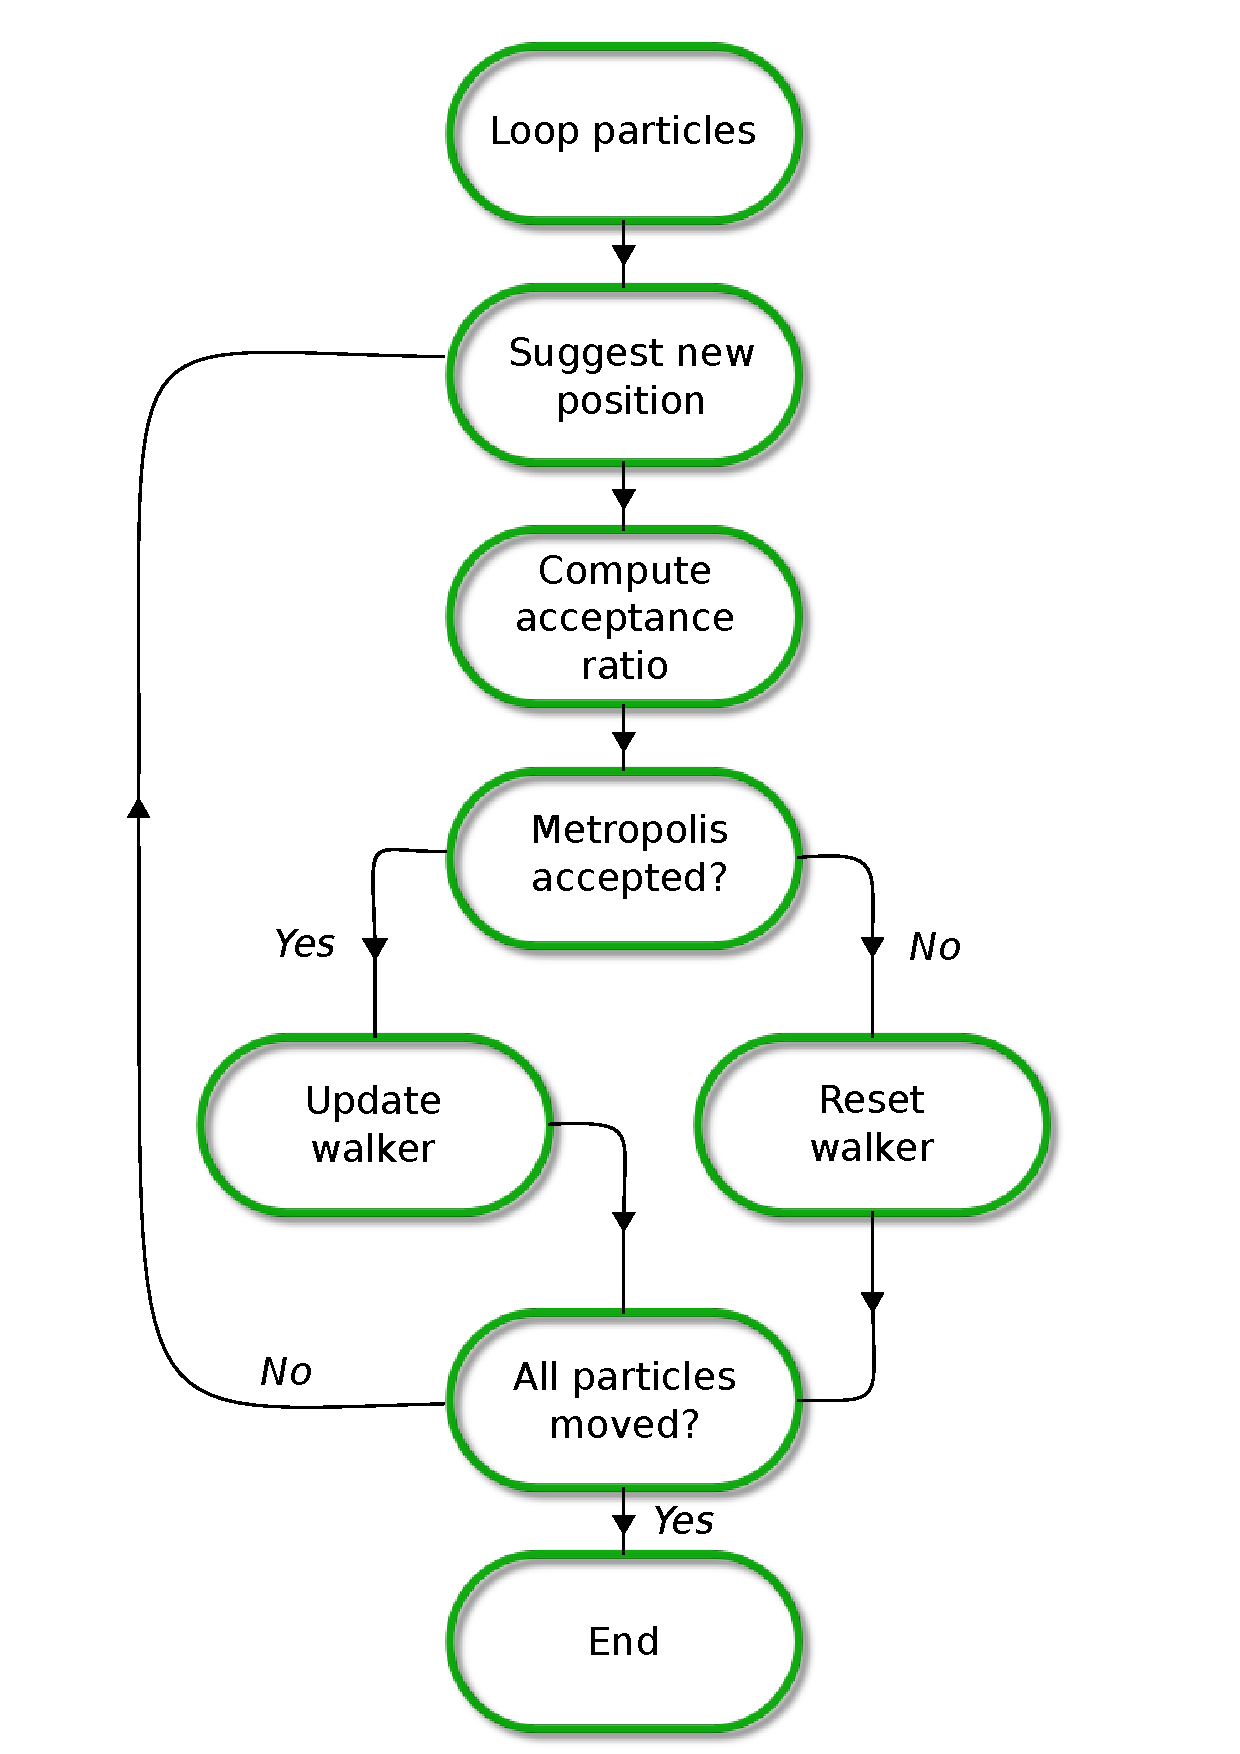
\includegraphics[scale=0.65]{../Graphics/DiffusionUML.pdf}
  \caption{Flow chart for iterating a walker through a single time step, i.e. simulation the application of the Green's function from Eq.~(\ref{eq:GDiff}) using the Metropolis algorithm. New positions are suggested according to the chosen diffusion model.}
  \label{fig:diffFlowChart}
 \end{center}
\end{figure}
\clearpage




\section{The Process of Branching}
\label{sec:branching}

In the previous section it became clear that the Metropolis test will guide the walkers to span the trial wave function. This implies that without further action, no changes to the distribution can be made, and the point of modeling the projection operator from Eq.~(\ref{eq:projOPonTrial}) is rendered useless. The important fact to include is that the branching Green's function from Eq.~(\ref{eq:branchFP}) and ~(\ref{eq:branchISO}) distribute weights to the walkers, effectively altering the spanned distribution. 

The process of branching in Quantum Monte-Carlo is simulated by the creation and destruction of walkers with probability equal to that of the branching Green's function \cite{abInitioMC}. The explicit shapes in case of isotropic diffusion (ISO) and Anisotropic (FP) is 

\begin{eqnarray}
 G_B^\mathrm{ISO}(i\,\rightarrow j) &=& e^{-\left(\frac{1}{2}\left[V(x_i) + V(x_j)\right] - E_T\right)\delta\tau}\label{eq:branchISO} \\
 G_B^\mathrm{FP}(i\,\rightarrow j) &=& e^{-\left(\frac{1}{2}\left[E_L(x_i) + E_L(x_j)\right] - E_T\right)\delta\tau}, \label{eq:branchFP}
\end{eqnarray}

where $E_L(x_i)$ is the energy evaluated in configuration $x_i$ (see Section \ref{sec:calcExpVals} for details). The three different scenarios which arise is

\begin{itemize}
 \item $G_B = 1$ : No branching, proceed main loop.
 \item $G_B = 0$ : The current walker is to be removed from the current ensemble.
 \item $G_B > 1$ : Make on average $G_B - 1$ replicas of the current walker.
\end{itemize}

Defining the following quantity allows for an efficient simulation of this behavior

\cfbox{1.1cm-10pt}{
\begin{equation}
 \overline{G}_B = \mathrm{floor}\left(G_B + a\right),\label{eq:gbMean}
\end{equation}
}


where $a$ is a uniformly distributed number on $[0,1)$. The chance that $\overline{G}_B = G_B + 1$ is then equal to $G_B - \mathrm{floor}(G_B)$. As an example, assume $G_B = 3.3$. The value of $\overline{G}_B$ is then either three or four, depending on whether $a < 0.7$ or not. The probability that $a<0.7$ is obviously $70\%$, implying that there is a $30\%$ chance that $\overline{G}_B$ is equal to four, and $70\%$ chance that is is equal to three. 

The process of branching is demonstrated in Fig. \ref{fig:branching}.

There are some programming challenges due to the fact that the number of walkers is not conserved, such as cleaning up inactive walkers and stabilizing the population across different computational nodes. For details regarding this, see the actual code reference at ref. \cite{libBorealisCode}. Isotropic diffusion is in practice never used with branching due to the singularities in the Coulomb interaction (see Eq.~(\ref{eq:branchISO})). This singularity may lead to large fluctuations in the walker population, the exact opposite to the optimal behavior.

\begin{figure}
 \begin{center}
  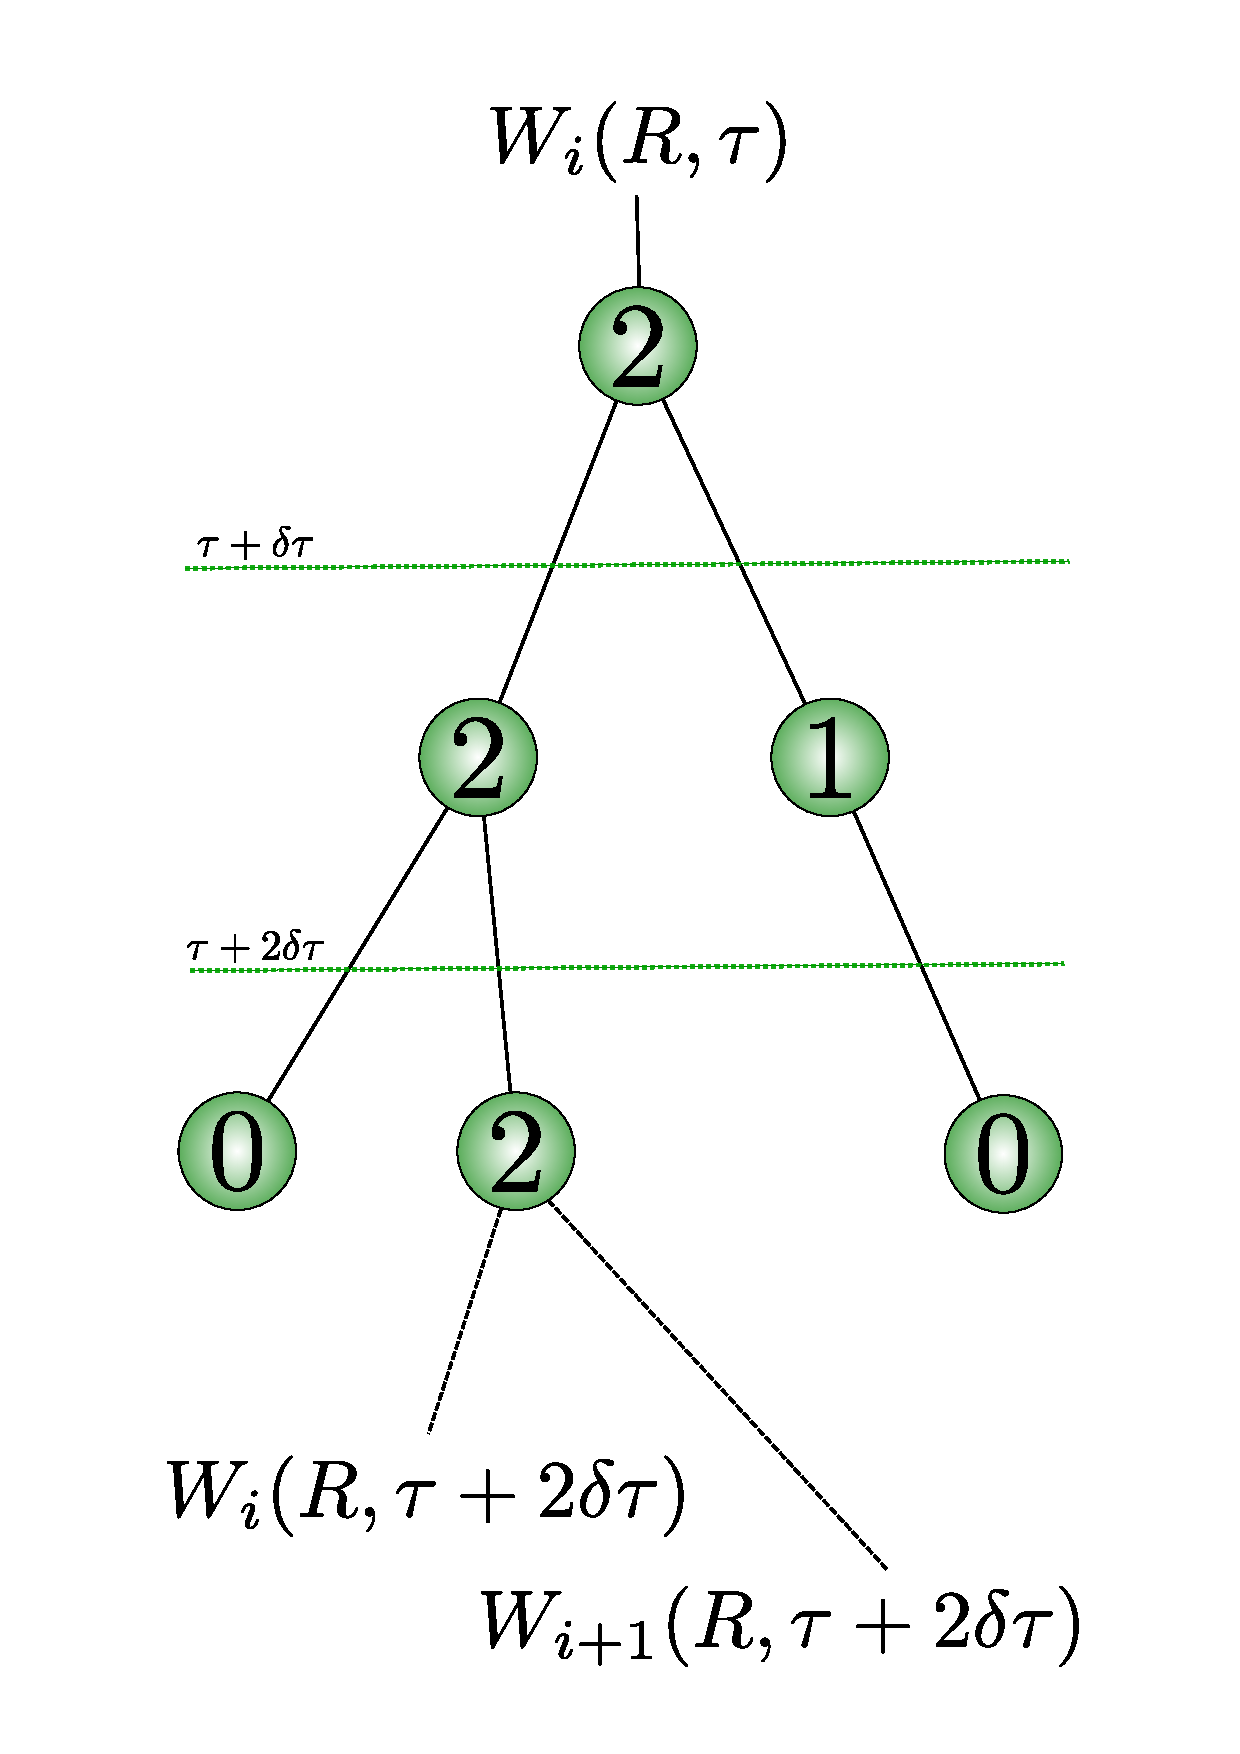
\includegraphics[scale=0.5]{../Graphics/branching.pdf}
  \caption{Branching illustrated. The initial walker $W_i(R, \tau)$ is branched according to the rules of Section \ref{sec:branching}. The numerical value inside the nodes represents $\overline{G}_B$ from Eq.~(\ref{eq:gbMean}). Each horizontal dashed line represent a diffusion step, i.e. a transition in time. Two lines exiting the same node represent identical walkers. After moving through the diffusion process, not two walkers should ever be equal (given that not all of the steps was rejected).}
  \label{fig:branching}
 \end{center}
\end{figure}
\clearpage

\section{The Trial Wave Function}
\label{sec:trialWF}

Recall Eq.~(\ref{eq:projOPonTrial}) and (\ref{eq:schrodGeneralSolution2}). The initial condition, $\Phi(\mathbf{r}, t_0) \equiv \PT$ ,
is in Quantum Monte-Carlo referred to as the trial wave function. Mathematically, any normalizable wave function can be chosen, whose overlap with the exact ground state wave function, $\Psi_0(x)$, is non-zero. If the overlap is zero, that is, $C_0=0$ in Eq.~(\ref{eq:ExactProjection}), the formalism breaks down, and no final state of convergence can be reached. On the other hand, the opposite scenario implies the opposite behavior; the closer $C_0$ is to unity, the more rapidly $\Psi_0(x)$ will become the dominant contribution to our distribution. 

In other words: The trial wave function should be chosen in such a manner that the overlap is optimized, i.e. close to unity. Since the exact ground state is unknown, this overlap has to be optimized based on educational guesses and by exploiting known requirements put on the exact ground state. This will be the focus in this section.  

Before getting into specifics, a few notes on many-body theory is needed. From this point on, all particles are assumed to be identical. For more information regarding basic Quantum Mechanics, I suggest reading in Ref. \cite{griffiths}. For mathematically rigid derivations of concepts, see ref. \cite{Sakurai:94}. More details regarding many-body theory can be found in Ref. \cite{Shavitt}. 

\subsection{Many-body Wave Functions}
\label{sec:manyBodyWFs}

Many-body theory arise from the existence of \textit{many-body interactions}, e.g. the Coulomb interaction between two particles. Nature operates with $N$-body interactions, however, it is overall safe to assume that the contributions beyond Coulomb decrease as the order of the interactions increase. If only one-body interactions were present, i.e. for non-interacting particles, the full system would decouple into $N$ single particle systems, rendering many-body theory redundant.

Finding the ground state is, not surprisingly, equivalent to solving the time-independent Schrödinger Equation (Eq.~(\ref{eq:schrodTimeIndie})) for the lowest energy eigenvalue

\begin{equation}
 \OP{H}\Psi_0(\mathbf{r}) = E_0\Psi_0(\mathbf{r}),
 \end{equation}
 
where $\mathbf{r} \equiv \{\mathbf{r}_1, \mathbf{r}_2, ..., \mathbf{r}_N\}$ represents every particle's position. Exact solutions to realistic many-body systems rarely exist, however, like in Section \ref{sec:statingDiff}, expanding the solution in a known basis $\Phi_k(\mathbf{r})$ is always legal, which reduces the problem into that of a \textit{coefficient hunt} 

\begin{equation}
\label{eq:manyBodyExp}
 \Psi_0(\mathbf{r}) = \sum_{k=0}^\infty C_k'\Phi_k(\mathbf{r}),
\end{equation}

where the primed coefficients should not to be confused with the previous coefficients expanding an arbitrary state in the $\Psi_i$ basis (see Eq.~(\ref{eq:schrodGeneralSolution2})). Different many-body methods, e.g. \textit{Hartree Fock}\footnote{Hartree-Fock is roughly a basis change from the non-interacting case into a basis which is orthogonal to one-particle excitations. The exact ground state wave function should be orthogonal to all excited states, so it's a fair approximation depending on the dominance of one-particle excitations in the given system.} and genetic algorithms, give rise to different ways of estimating these coefficients, however, certain concepts are necessarily common, for instance truncating the basis at some level, $K$:

\begin{equation}
 \Psi_0(\mathbf{r}) = \sum_{k=0}^K \tilde{C}_k'\Phi_k(\mathbf{r}), \label{eq:manybodyWFexp}
\end{equation}

where $ \tilde{C}_k' \ne  C_k'$ unless $K$ tends to infinity, however, it is overall safe to assume that the value of the coefficients decrease as $k$ increase (given a reasonable ordering, more on this shortly). 

The many-body basis elements $\Phi_k(\mathbf{r})$ are constructed using $N$ elements from a basis of single particle wave functions (or \textit{orbitals} for short) $\phi_n(\mathbf{r}_i)$, combined in different ways. The process of calculating basis elements often boils down to a combinatoric exercise involving combinations of orbitals.

Imagine electrons surrounding a nucleus, i.e an atom. A single electron occupying a state with quantum numbers $n$ at a position $\mathbf{r}_i$ is then described by the orbital $\phi_n(\mathbf{r}_i)$. Each unique\footnote{Two wave functions are considered equal if they differ by nothing but a phase factor.} configuration of electrons (in terms of $n$) will give rise to one unique $\Phi_k(\mathbf{r})$. In other words, the complete basis of $\Phi_k(\mathbf{r})$ is described by the collection of all possible excited states and the ground state. $\Phi_0(\mathbf{r})$ is the ground state of the atom, $\Phi_1(\mathbf{r})$ has one electron exited to a higher shell, $\Phi_2(x)$ has another, and so on. See Fig.~\ref{fig:AtomicOrbitals} for a demonstration of this. The ordering of the terms in Eq.~(\ref{eq:manybodyWFexp}) are thus chosen to represent higher and higher excitations, i.e. the states has higher and higher energy eigenvalues.

\begin{figure}
 \begin{center}
  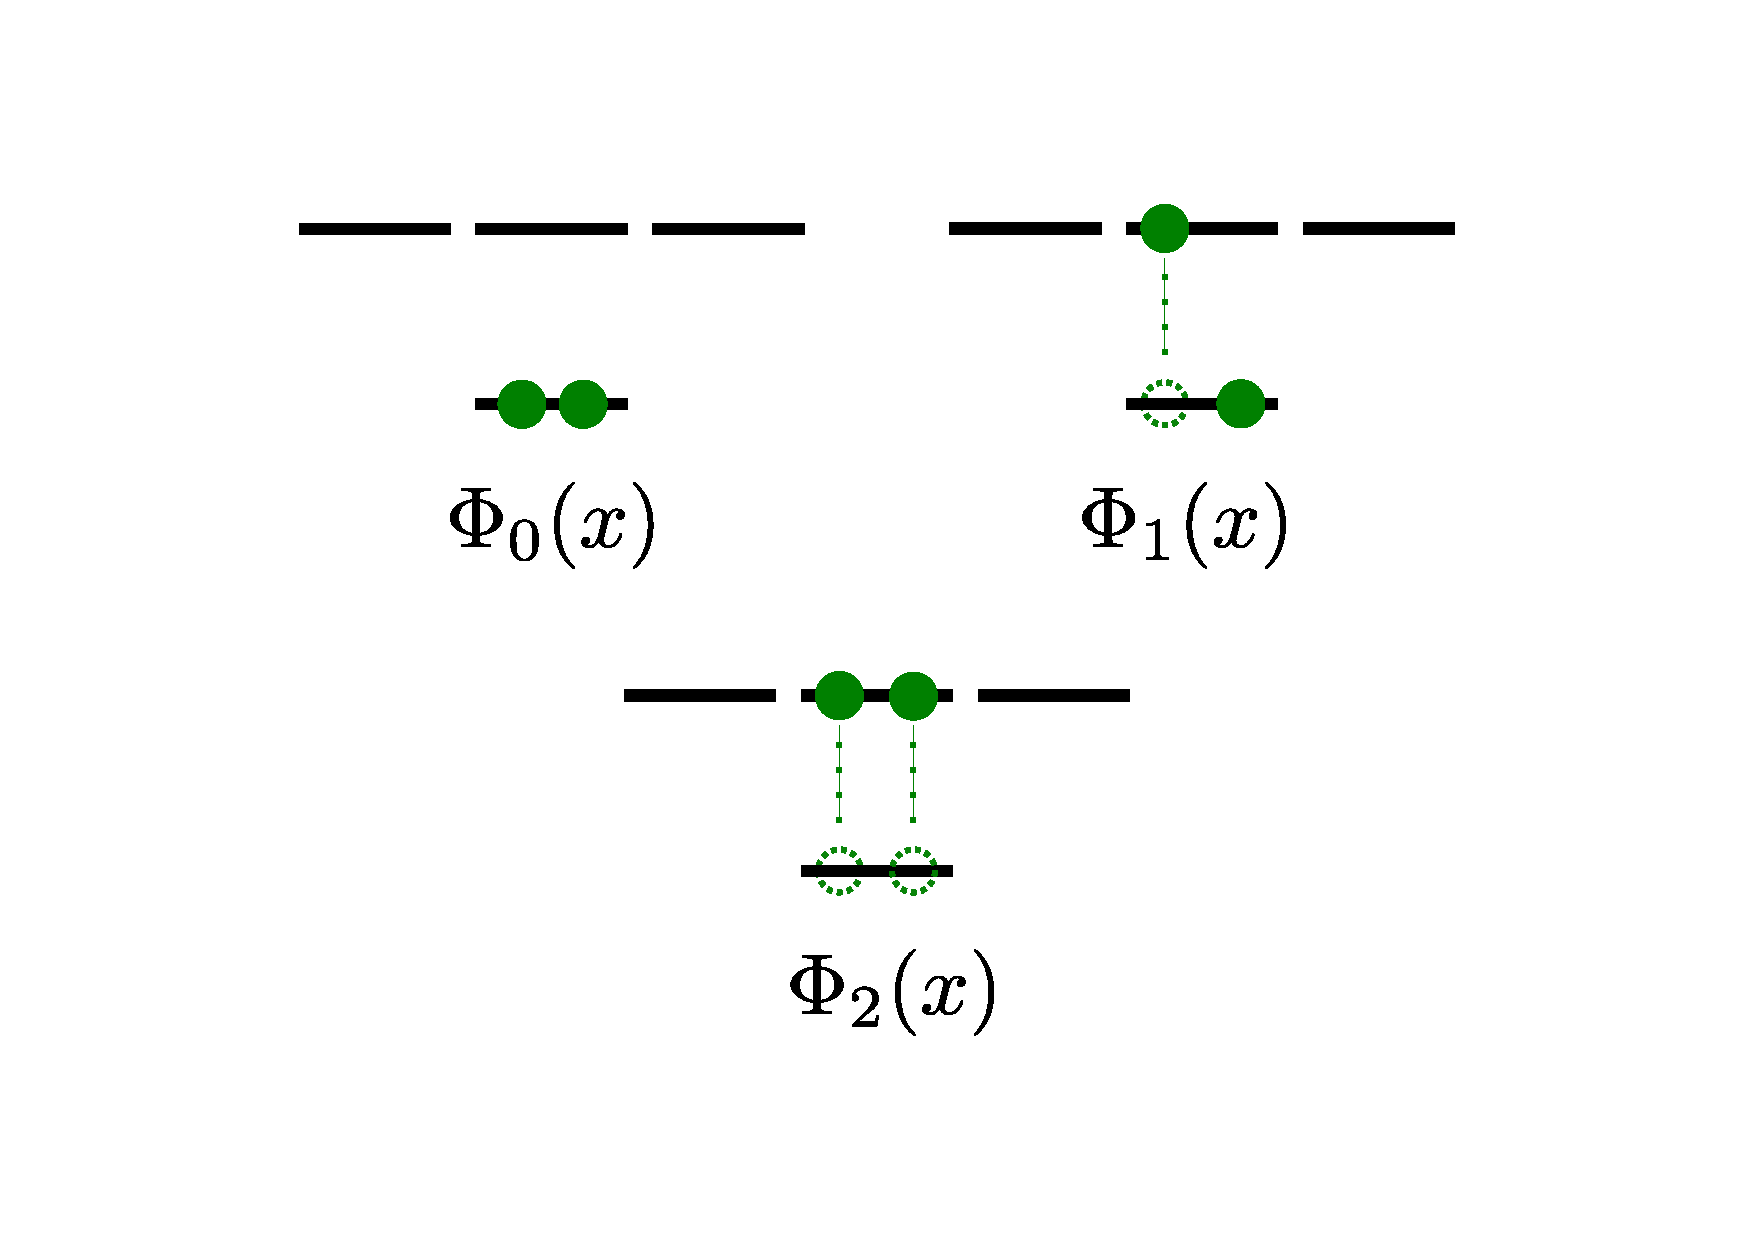
\includegraphics[scale=0.5]{../Graphics/shellStructure.pdf}
  \caption{Three different electron configurations in an shell structure making up three different $\Phi_k(\mathbf{r})$, i.e. constituents of the many-body basis described in Eq.~(\ref{eq:manybodyWFexp}). An electron (solid dot) is represented by e.g. the orbital $\phi_{1s}(\mathbf{r}_1)$.}
  \label{fig:AtomicOrbitals}
 \end{center}
\end{figure}

To summarize, constructing an approximation to an unknown many-body ground state wave function involves three steps:

\begin{center}
\begin{tabular}{l|l}
 \textbf{Step one}   &  Choose a basis of orbitals $\phi_n(\mathbf{r}_i)$, e.g. hydrogen states. \\
 \textbf{Step two}   &  Construct $\Phi_k(\mathbf{r})$ from $N\times$ $\phi_n(\mathbf{r}_i)$.   \\
 \textbf{Step three} &  Construct $\Psi_0(\mathbf{r})$ from $K\times$ $\phi_k(\mathbf{r})$.     \\
\end{tabular}
\end{center}

The last step is well described by Eq.~(\ref{eq:manybodyWFexp}), but is seldom necessary to perform explicitly; expressions involving the approximated ground state wave function is given in terms of the constituent $\Phi_k(\mathbf{r})$ elements and their coefficients.

\subsubsection{Step one in detail}

The Hamiltonian of a $N$-particle system is 

\begin{equation}
 \OP{H} = \OP{H}_0 + \OP{H}_\mathrm{I},
\end{equation}

where $\OP{H}_0$ and $\OP{H}_\mathrm{I}$ are respectively the one-body - and the many-body Hamiltonian. As mentioned in the introduction, the many-body interactions in $\OP{H}_\mathrm{I}$ are truncated at the level of Coulomb. The one-body term consist of the external potential $\OP{u}_\mathrm{ext}(\mathbf{r}_i)$ and the kinetic terms $\OP{t}(\mathbf{r}_i)$ for all particles.

\begin{eqnarray}
 \OP{H}_0 &=& \sum_{i=1}^N \OP{h}_0(\mathbf{r}_i) \\
          &=& \sum_{i=1}^N \OP{t}(\mathbf{r}_i) + \OP{u}_\mathrm{ext}(\mathbf{r}_i) \nonumber\\
 \OP{H}_\mathrm{I} &\simeq& \sum_{i<j=1}^N \OP{v}(r_{ij}) \\
          &=& \sum_{i<j=1}^N \frac{1}{r_{ij}},  \nonumber
\end{eqnarray}

where $r_{ij} = |\mathbf{r}_i - \mathbf{r}_j|$ is the distance between two particles.

In order to optimize the overlap $C_0$, the single particle orbitals are commonly chosen to be the solutions of the non-interacting case (given that they exist)

\begin{equation}
\label{eq:orbitalEigenEq}
 \OP{h}_0(\mathbf{r}_i)\phi_n(\mathbf{r}_i) = \epsilon_n\phi_n(\mathbf{r}_i).
\end{equation}

If no such choice can be made, choosing e.g. free-particle solutions, Laguerre polynomials etc. is the general strategy. However, in this case, the expansion truncation $K$ needs to be higher in order to achieve a satisfying overlap.  


\subsubsection{Step two in detail}

In the case of \textit{fermions}, i.e. half-integer spin particles like electrons, protons, etc., $\Phi_k(\mathbf{r})$ is an anti-symmetric function\footnote{Interchanging two particles in an anti-symmetric wave function will reproduce the state changing only the sign.} on the form of a determinant: The \textit{Slater determinant}. The shape of the determinant is given in Eq.~(\ref{eq:SlaterDeterminantExplicit}). The anti-symmetry is a direct consequence of the \textit{Pauli Exclusion Principle}: At any given time, two fermions cannot occupy the same state. 

Bosons on the other hand have symmetric wave functions (see Eq.~(\ref{eq:BosonicWFExplicit})), which in many ways are easier to deal with because of the lack of an exclusion principle. In order to keep the terminology less abstract and confusing, from here on, the focus will be on systems of fermions.

\cfbox{1.2cm-6pt}{
\begin{eqnarray}
\label{eq:SlaterDeterminantExplicit}
\Phi_0^\mathrm{AS}(\mbf{r}_1, \mbf{r}_2, ..., \mbf{r}_N) &\propto& \sum_\mathrm{P} (-)^\mathrm{P} \OP{P}\phi_1(\mbf{r}_1)\phi_2(\mbf{r}_2)\,...\,\phi_N(\mbf{r}_N) \nonumber\\
\nonumber\\
&=&\left| \begin{array}{cccc}
\phi_1(\mbf{r}_1) & \phi_2(\mbf{r}_1)& \cdots & \phi_N(\mbf{r}_1) \\
\phi_1(\mbf{r}_2) & \phi_2(\mbf{r}_2)& \cdots & \phi_N(\mbf{r}_2) \\
\vdots & \vdots& \ddots & \vdots \\
\phi_1(\mbf{r}_N) & \phi_2(\mbf{r}_N)& \cdots & \phi_N(\mbf{r}_N) \\
 \end{array} \right| \\
\nonumber\\
\nonumber\\
 \label{eq:BosonicWFExplicit}
 \Phi_0^\mathrm{S}(\mbf{r}_1, \mbf{r}_2, ..., \mbf{r}_N) &\propto& \sum_\mathrm{P} \OP{P}\phi_1(\mbf{r}_1)\phi_2(\mbf{r}_2)\,...\,\phi_N(\mbf{r}_N)
\end{eqnarray}
}

The permutation operator $\OP{P}$ is simply a way of writing \textit{in any combination of particles and states}, hence the combinatoric exercise mentioned previously. Any combination of $N$ orbital elements $\phi_n(\mbf{r}_i)$ can be used to produce different $\Phi_k(\mathbf{r})$. For illustrative purposes, and for the purpose of this thesis in general where a single determinant ansatz is used, only the ground state has been presented.  

\subsubsection{Dealing with correlations}

The contributions to the ground state on the right-hand side in Eq.~(\ref{eq:manyBodyExp}) for $k>0$ are referred to as \textit{correlation} terms. Given that the orbital wave functions are chosen by Eq.~(\ref{eq:orbitalEigenEq}), the existence of the correlation terms, i.e. $C_k' \ne 0$ for $k>0$, follows as a direct consequence of the many-body interaction, $H_\mathrm{I}$, hence the name.

As an example, imagine performing an energy calculation with two particles being infinitely close; the Coulomb singularity will cause the energy to blow up. However, if the calculations are performed using the exact wave function, the diverging terms will cancel out; the energy is independent of the position. 

In other words, incorporating the correct correlated wave function will result in a cancellation in the diverging terms as walkers approach regions where the many-body interactions are singular, a property of exact ground states which can be enforced upon the approximation to further optimize the overlap. 

These criteria are called \textit{Cusp Conditions}, and serve as a powerful guide when it comes to selecting a trial wave function. 





\subsection{Choice of Trial Wave function}
\label{sec:ChoiceTrialWF}

To recap, choosing the trial wave function boils down to optimizing the overlap $C_0 = \braket{\Psi_0}{\Psi_T}$ using a priori knowledge about the system at hand. As discussed previously, the optimal choice of single particle basis is eigenfunctions of the non-interacting case (given that they exist). Starting from Eq.~(\ref{eq:manybodyWFexp}), from here on referred to as the \textit{spatial wave function}, the first step is to make sure the cusp conditions are obeyed.

Introducing the correlation functions $f(r_{ij})$, where $r_{ij}$ is the relative distance between particle $i$ and $j$, the general ansatz for the trial wave function becomes

\begin{equation}
\label{eq:firstAnzatsTWF}
 \Psi_T(\mbf{r}_1, ..., \mbf{r}_N) = \Big[\sum_{k=0}^K C_k\Phi_k(\mbf{r}_1, ..., \mbf{r}_N)\Big]\prod_{i<j}^Nf(r_{ij}).
\end{equation}

The idea is now to choose $f(r_{ij})$ in such a way that the cusp conditions are obeyed. This should, in light of previous discussions, reduce the amount of terms needed in the spatial wave function to obtain a satisfying overlap.

\subsubsection{Explicit shapes}

Several models for the correlation function exist, however, some are less practical than others. An example given in ref. \cite{abInitioMC} demonstrates this nicely: Hylleraas presented the following correlation function 

\begin{equation}
 f(r_{ij})_\mathrm{Hylleraas} = e^{-\frac{1}{2} (r_i + r_j)}\sum_k d_k(r_{ij})^{a_k} (r_i + r_j)^{b_k}(r_i - r_j)^{e_k},
\end{equation}

where all $k$-subscripted parameters are free. Calculating the helium ground state energy using this correlation function with nine terms yields a four decimal precision. Eight digit precision is achieved by including almost 1078 terms. For the purpose of Quantum Monte-Carlo this is beyond overkill: Three decimal precision is obtained using a single free parameter (see the results for Atoms in Table \ref{tab:AtomsRes}). 

A commonly used correlation function in studies involving few variational parameters is the \textit{Padé Jastrow} function (skipping some redundant indices) 

\begin{eqnarray*}
 \prod_{i<j}^Nf(r_{ij}) &=& \exp(U) \\
         U &=&  \sum_{i<j}^N\left(\frac{\sum_k a_kr_{ij}^k}{1 + \sum_k \beta_kr_{ij}^k}\right) + \sum_i^N\left(\frac{\sum_k a'_kr_i^k}{1 + \sum_k \alpha_kr_i^k}\right).
\end{eqnarray*}

For systems where the correlations are relatively well behaving, it is custom to drop the second term, and keep only the $k=1$ term, which yields

\begin{equation}
 \label{eq:jastrow}
 f(r_{ij}; \beta) = \exp\left(\frac{a_{ij} r_{ij}}{1 + \beta r_{ij}}\right),
\end{equation}

where $\beta$ is a variational parameter, and $a_{k=1} \equiv a_{ij}$ is a constant depending on the relative spin-orientation of particles $i$ and $j$ tuned in such a way that the cusp conditions are obeyed. For three dimensions, $a_{ij} = 1/4$ or $a_{ij} = 1/2$ depending on whether or not the spins of $i$ and $j$ are parallell or anti parallell respectively\cite{abInitioMC}. For two dimensions, the values are $a_{ij}=1/3$ (parallell) or $a_{ij}=1$ (anti-parallel)\cite{larseivind}. This is the correlation function used for all systems this thesis.

Shifting the focus back to the spatial wave function, in the case of a fermionic system, the evaluation of a $N\times N$ Slater determinant severely limits the efficiency of many-particle simulations. However, assuming the Hamiltonian to be spin-independent, the eigenstates for different spin eigenvalues can be assumed identical, which allows the spatial wave function to be split in two: One part for each spin eigenvalue. A detailed derivation of this is given in the appendix of Ref. \cite{QMCPHD2008}. Assuming spin-half particles yields

\begin{equation}
 \Psi_T(\mathbf{r}; \beta) = \Big[\sum_{k=0}^K C_k'\tilde\Phi_k(\mbf{r}_1, ..., \mbf{r}_{\frac{N}{2}})\tilde\Phi_k(\mbf{r}_{\frac{N}{2}-1}, ..., \mbf{r}_{N})\Big]\prod_{i<j}^Nf(r_{ij}; \beta). \label{eq:splitSlater}
\end{equation}

Due to the identical nature of the particles, they may be arbitrarily ordered. For simplicity, the first half represents spin up, and the second half spin down. The spin up determinant will from here on be labeled $D^\uparrow$, and the spin down one $D^\downarrow$. Stitching everything together yields the following explicit shape for a spin-independent Hamiltonian using a one-parameter Padé Jastrow function

\cfbox{1.5cm-8pt}{
\begin{equation}
\label{eq:MultiDeterminantTWF}
 \Psi_T(\mbf{r}_1, ..., \mbf{r}_N; \beta) = \sum_{k=0}^K C_k' D^\uparrow_kD^\downarrow_k\prod_{i<j}^Nf(r_{ij}; \beta).
\end{equation}
}

This shape is referred to as a \textit{Multi-determinant} trial wave function. 

\subsubsection{Limitations}

Depending on the complexity of the system at hand, more complicated trial wave functions might be needed to obtain reasonable convergence. However, it is important to distinguish between simply integrating a trial wave function, and performing the full diffusion calculation. As a reminder: Simple integration will not be able to alter the distribution; what you have is what you get. Solving the diffusion problem, on the other hand, will alter the distribution from that of the trial wave function ($\tau = 0$) into a distribution closer to the exact wave function by Eq.~(\ref{eq:schrodGeneralSolution2}). 

Because of this fact, limitations due to the trial wave function in full\footnote{``Full'' in the sense that all Green's functions are applied. As will be revealed later, VMC corresponds to a standard importance sampled Monte-Carlo integration by omitting the branching process.} QMC is far less than what is the case of standard Monte-Carlo integration. A more complex trial wave function might convergence faster, but at the expense of being more CPU-intensive. This implies that CPU-time per walker can be traded for convergence time. For systems of many particles, CPU-time per walker needs to be as low as possible in order to get the computation done in a reasonable amount of time, i.e., the choice of trial wave function needs to be done in light of the system at hand, and the specific aim of the computation. 

On the other hand, increasing the number of particles in the system may cause the generic trial wave function to be relatively worse than in the case with fewer particles. This is demonstrated in Ref. \cite{UmrigarMolecules} where calculations for $\mathrm{F}_2$ (18 particles) needs an increase in the number of determinants to achieve a result with the same precision as calculations for $\mathrm{O}_2$ (16 particles).  

\subsubsection{Single Determinant Trial Wave function}

In the case of well-behaving systems, a single determinant (with the Jastrow factor) is a reasonable approximation. This simplicity opens up the possibility of simulating large systems efficiently (more details regarding this is given in Section \ref{sec:optSingleSlater}). 

In order to further optimize the overlap with the exact wave function, a variational parameter $\alpha$ is introduced in the spatial part (in addition to $\beta$from Eq.~(\ref{eq:jastrow}))

\cfbox{8mm}{
\begin{equation}
\label{eq:singleDeterminantTWF}
 \Psi_T(\mbf{r}_1, ..., \mbf{r}_N; \alpha, \beta) = D^\uparrow(\alpha)D^\downarrow(\alpha)\prod_{i<j}^Nf(r_{ij}; \beta).
\end{equation}
}

Determining optimal values for the variational parameters will be discussed in Section \ref{sec:selectingOptVarPar}. If the introduction of the variational parameter was redundant, optimizations would simply yield $\alpha=1$. 


\subsection{Selecting Optimal Variational Parameters}
\label{sec:selectingOptVarPar}

All practical ways of determining the optimal values of the variational parameters originate from the same powerful principle: \textit{The Variational Principle}. The easiest way of demonstrating the principle is to evaluate the expectation value of the energy, using an approach similar to what used in Eq.~(\ref{eq:schrodGeneralSolution2})

\begin{eqnarray*}
 E_0 &=& \bra{\Psi_0}\OP{H}\ket{\Psi_0}  \\
 E   &=& \bra{\Psi_T(\alpha, \beta)}\OP{H}\ket{\Psi_T(\alpha, \beta)}\\
     &=& \sum_{kl} C_k^\ast C_l \underbrace{\bra{\Psi_k}\OP{H}\ket{\Psi_l}}_{E_k\delta_{kl}} \\
     &=& \sum_k |C_k|^2E_k
\end{eqnarray*}

Just as with the projection operator, introducing $E_k = E_0 + \delta E_k$ where $\delta E_k \ge 0$ will simplify the arguments

\begin{eqnarray*}
 E   &=& \sum_k |C_k^2| (E_0 + \delta E_k) \\
     &=& E_0 \underbrace{\sum_k |C_k^2|}_{1} + \underbrace{\sum_k |C_k|^2\delta E_k}_{\ge 0} \\
     &\ge& E_0
\end{eqnarray*}

The conclusion is remarkable: No matter which trial wave function is used, the result will always be greater or equal to the exact ground state energy. This implies that the problem of choosing variational parameters comes down to a minimization problem in the parameters space (assuming no maxima exist for finite values of the parameters)

\begin{equation}
\label{eq:varMin}
\frac{\partial \langle E\rangle}{\partial \alpha_i} = \frac{\partial}{\partial \alpha_i}\bra{\Psi_T(\alpha_i)}\OP{H}\ket{\Psi_T(\alpha_i)} = 0
\end{equation}

In order to work with Eq.~(\ref{eq:varMin}) in practice, it needs to be rewritten it in terms of known values. Since our wave function is dependent on the variational parameter, the normalization factor needs to be included in the expression of the expectation value

\newcommand{\Norm}{\braket{\Psi_T(\alpha_i)}{\Psi_T(\alpha_i)}}

\begin{eqnarray*}
 \frac{\partial \langle E\rangle}{\partial \alpha_i}  &=& \frac{\partial}{\partial \alpha_i} \frac{\bra{\Psi_T(\alpha_i)}\OP{H}\ket{\Psi_T(\alpha_i)}}{\Norm} \\
 &=& \frac{\left(\bra{\Psi_T(\alpha_i)}\frac{\partial}{\partial \alpha_i}\OP{H}\ket{\Psi_T(\alpha_i)} + \bra{\Psi_T(\alpha_i)}\OP{H}\frac{\partial}{\partial \alpha_i}\ket{\Psi_T(\alpha_i)}\right)}{\Norm^2}\Norm \\
 &-& \bra{\Psi_T(\alpha_i)}\OP{H}\ket{\Psi_T(\alpha_i)}\frac{\left(\bra{\Psi_T(\alpha_i)}\frac{\partial}{\partial \alpha_i}\right)\ket{\Psi_T(\alpha_i)} + \bra{\Psi_T(\alpha_i)}\left(\frac{\partial}{\partial \alpha_i}\ket{\Psi_T(\alpha_i)}\right)}{\Norm^2},\\
\end{eqnarray*}

where the product and division rules for derivatives has been applied. The Hamiltonian does not depend on the variational parameters, hence both terms in the first expansion is equal. Cleaning up the expression yields

\cfbox{2cm-10pt}{
\begin{eqnarray}
 \frac{\partial \langle E\rangle}{\partial \alpha_i} &=& 2\left(\frac{\bra{\Psi_T(\alpha_i)}\OP{H}\frac{\partial}{\partial \alpha_i}\ket{\Psi_T(\alpha_i)}}{\Norm} - \langle E \rangle\frac{\bra{\Psi_T(\alpha_i)}\frac{\partial}{\partial \alpha_i}\ket{\Psi_T(\alpha_i)}}{\Norm} \right) \nonumber \\
  &=& 2\left(\left< E \frac{\partial \Psi_T}{\partial \alpha_i} \right> -\left< E\right>\left<\frac{\partial \Psi_T}{\partial \alpha_i} \right> \right) \label{eq:varParGrad} \\
  \nonumber
\end{eqnarray}
}

In the case of $\Psi_T(\mathbf{r}; \alpha_i)$ being represented by a Slater determinant, the relationship between the variational derivative of the determinant and the variational derivative of the single particle orbitals $\phi_n(\mathbf{r}_i; \alpha_i)$ is

\cfbox{2cm-5pt}{
\begin{equation}
 \frac{\partial \Psi_T(\mathbf{r}; \alpha_i)}{\partial \alpha_i} = \sum_{p=1}^N\sum_{q=0}^{N/2} \phi_q(\mathbf{r}_p; \alpha_i) \left[\frac{\partial \phi_q(\mathbf{r}_p; \alpha_i)}{\partial \alpha_i}\right]\mathbf{S}^{-1}_{qp},
\end{equation}
}

where $\mathbf{S}^{-1}_{qi}$ is the inverse of the Slater matrix, which will be introduced in more detail in Section \ref{sec:optSlaterRat}. 

Using these expressiosn for the \textit{variational energy gradient}, the derivatives can be calculated exactly the same way as for e.g. the energy. The gradient can then be used to move in the direction of the variational minimum in Eq.~(\ref{eq:varMin}). 

This strategy give rise to numerous ways of finding the optimal parameters, such as using the well known Newton's method, conjugate gradient methods \cite{golub1996matrix}, steepest descent (similar to Newton's method), and many more. 
The method implemented for this thesis is called \textit{Adaptive Stochastic Gradient Descent}, and is an efficient iterative algorithm for seeking the variational minimum. The gradient descent methods will be covered in Section \ref{sec:GradientDescent}.

\subsection{Calculating Expectation Values}
\label{sec:calcExpVals}

The expectation value of an operator $\OP{O}$ is obtained by sampling \textit{local} values, $O_L(x)$

\begin{eqnarray}
 \bra{\Psi_T}\OP{O}\ket{\Psi_T} &=& \int \Psi_T(x)^\ast \OP{O} \Psi_T(x)\mathrm{d}x \nonumber\\
                                &=& \int |\Psi_T|^2\left(\frac{1}{\Psi_T(x)}\OP{O}\Psi_T(x)\right)\mathrm{d}x \nonumber\\
                                &=& \int |\Psi_T|^2 O_L(x)\mathrm{d}x \\
                         O_L(x) &=& \frac{1}{\Psi_T(x)}\OP{O}\Psi_T(x)           
\end{eqnarray}

Discretizing the integral yields 

\begin{equation}
 \bra{\Psi_T}\OP{O}\ket{\Psi_T} \equiv \Exp{O} \simeq \frac{1}{n}\sum_{i=1}^n O_L(x_i) \equiv \overline{O},
\end{equation}

where $x_i$ is a random variable taken from distribution of the trial wave function. The \textit{ensemble average},  $\Exp{O}$ will, given ergodicity, equal the estimated average $\overline{O}$ in the limit $n\rightarrow\infty$, i.e.

\begin{equation}
 \label{eq:MeanVStrueExp}
 \Exp{O} = \lim_{n\to\infty} \overline{O} = \lim_{n\to\infty}\frac{1}{n}\sum_{i=1}^n O_L(x_i)
\end{equation}


In the case of the energy estimation, this implies that once the walkers reach equilibrium, local values can be sampled based on the walker configurations $\mathbf{r}_i$ (remember that Metropolis ensures that the walkers follow $|\PT|^2$). In the case of energies, the explicit expression becomes

\begin{equation}
 \langle E \rangle \simeq \frac{1}{n}\sum_{i=1}^n \left(\frac{1}{\Psi_T(x_i)}\left(-\frac{1}{2}\nabla^2\right)\Psi_T(x_i) + V(x_i)\right)
\end{equation}

Incorporating the branching Green's function $G_B$ into the above equation is covered in the DMC section.

\subsection{Normalization}

Every explicit calculation using the trial wave function in Quantum Monte-Carlo involves taking ratios. Calculating ratios implies a cancellation in the normalization factors. Eq.~(\ref{eq:MetroGeneralGreen}) from the Metropolis section, the Quantum Force in the Fokker-Planck equation, and the sampling of local values describes in the previous section demonstrates exactly this; everything involves ratios.

Not having to normalize our wave functions saves us a lot of CPU-time, but it also relieves us of complicated normalization factors in our single particle basis expressions; any constants multiplying $\phi_n(x_i)$ in Eq.~(\ref{eq:SlaterDeterminantExplicit}) and Eq.~(\ref{eq:BosonicWFExplicit}), can be taken outside the sum over permutations, and will hence cancel when the ratio between two wave functions constituting of the same single particle orbitals are computed. 

Note, however, that this argument is valid for single determinant wave functions only. In the case of multi-determinants trial wave functions, the normalization factors from the single particle basis elements will be absorbed by the respective determinant's coefficient $C_k$, and is hence obsolete in this case as well. 

\section{Gradient Descent Methods}
\label{sec:GradientDescent}

The direction of a gradient serves as a guide to extremal values. Gradient descent, also called steepest descent\footnote{In literature, steepest - and gradient descent are sometimes referred to as being different. However, for simplicity these will not be differentiated.}, is a family of minimization methods using this property of gradients in order to backtrace a local minimum in the vicinity of an initial guess. 

\subsection{General Gradient Descent}

Seeking maxima or minima is simply a question of whether the positive or negative direction of the gradient is followed.
Imagine a function $f(x)$, with a minimum residing at $x=x_m$. The information at hand is then

\begin{eqnarray}
 \nabla f(x_m) &=& 0 \\
 \nabla f(x_m - \mathrm{d}x) &<& 0 \\
  \nabla f(x_m + \mathrm{d}x) &>& 0
\end{eqnarray}

where $\mathrm{d}x$ is a infinite decimal displacement. 

\begin{figure}
 \begin{center}
  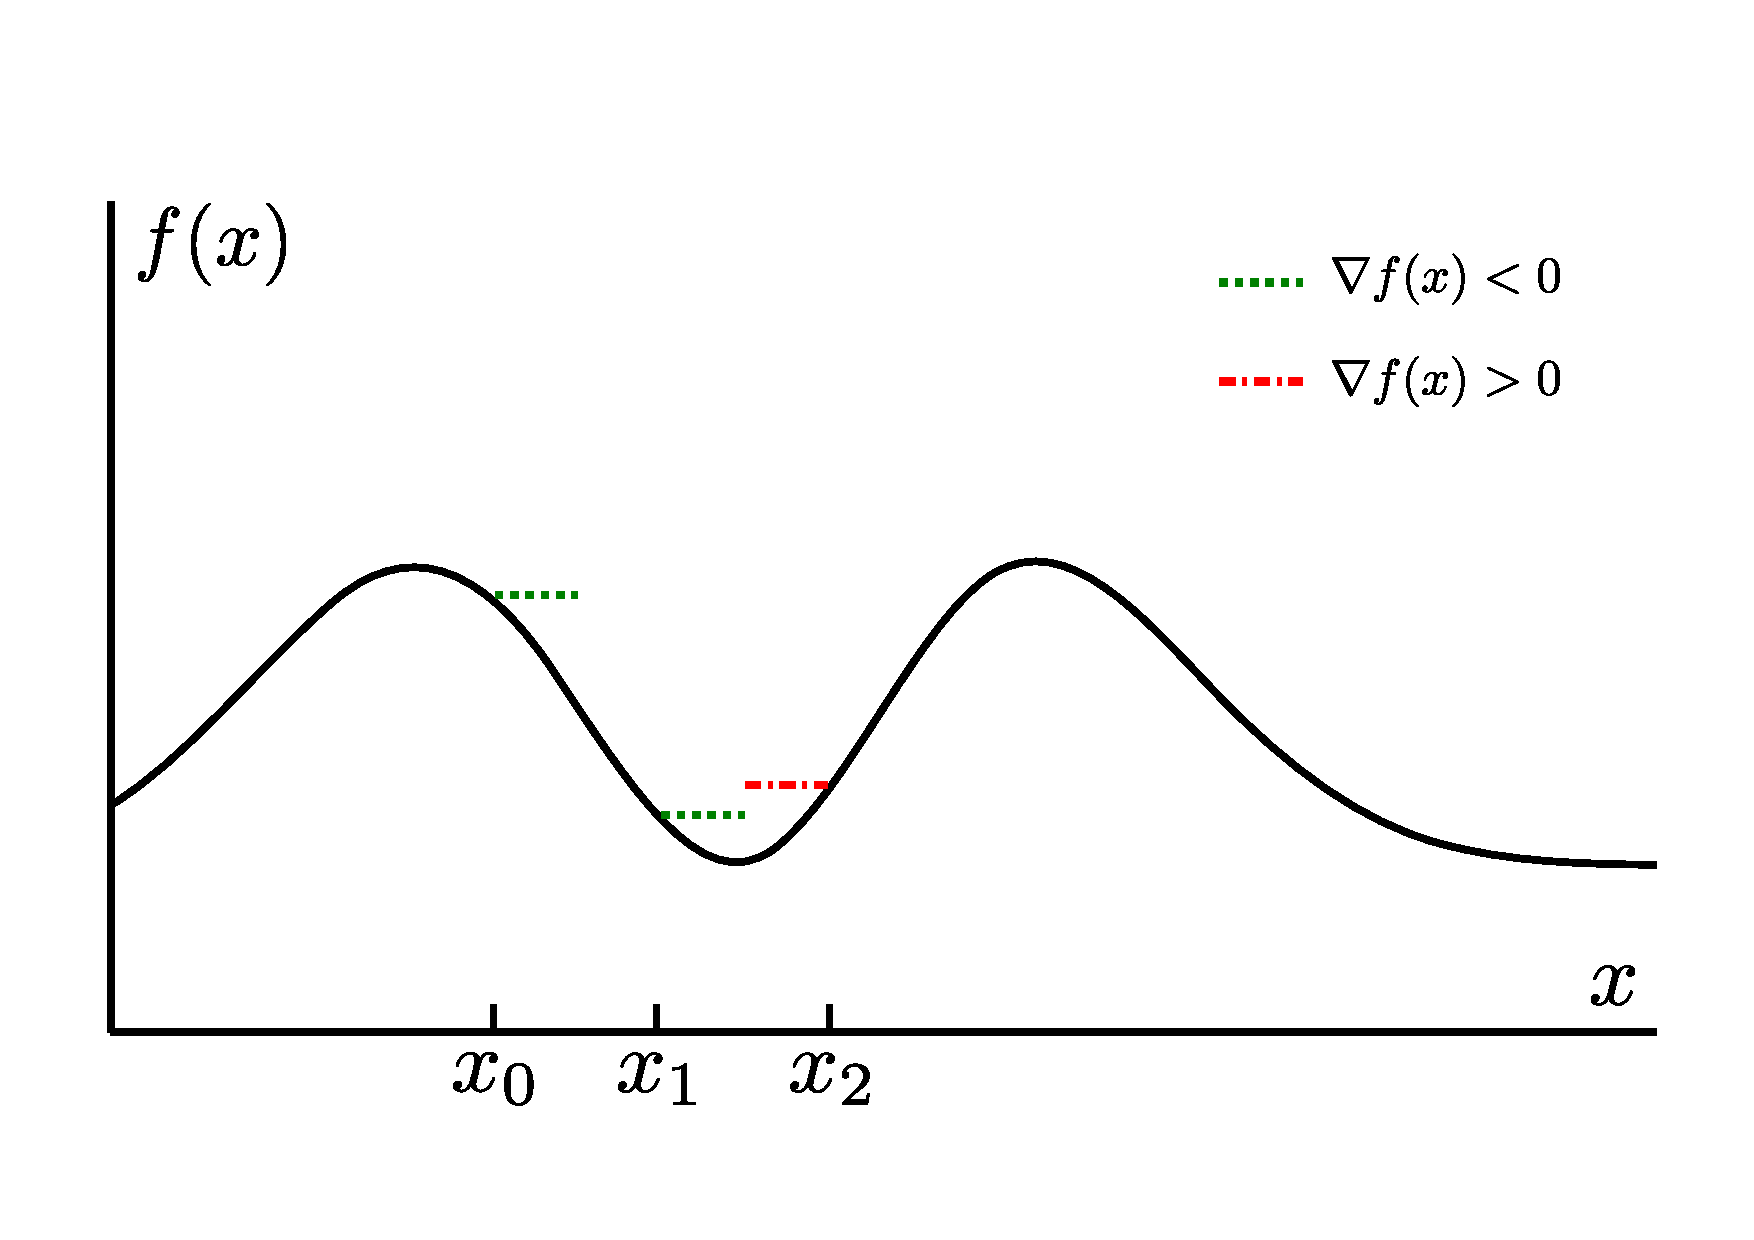
\includegraphics[scale=0.3]{../Graphics/SGD.pdf}
  \caption{Two steps of a one dimensional Gradient Descent process. Steps are taken in the direction of the negative gradient (indicated by dotted lines).}
  \label{fig:SGD}
 \end{center}
\end{figure}

As an example, imagine starting from an initial guess $x_0$. The direction of the gradient is then calculated and followed (backwards) a number of steps. From Fig. \ref{fig:SGD} and the previous equations, it is clear that crossing the true minimum induces a sign change in the gradient. The brute force way of minimizing is to simply end the calculation at this point, however, this would require a extreme amount of very small steps in order to achieve good precision. 

The difference equation describing the steps from the previous paragraph would be

\begin{equation}
 x_{i+1} = x_i - \delta\frac{\nabla f(x_i)}{|\nabla f(x_i)|}
\end{equation}


An improved algorithm would be to continue iterating even though the minimum is crossed, however, this would cause the constant step-length algorithms to oscillate between two points, e.g. $x_1$ and $x_2$ in Fig. \ref{fig:SGD}. To counter this, a changing step length $\delta_i$ is introduced

\cfbox{2.2cm-8pt}{
\begin{equation}
\label{eq:SGD}
  x_{i+1} = x_i - \delta_i\nabla f(x_i)
\end{equation}
}


All gradient/steepest descent methods are in principle described by Eq.~(\ref{eq:SGD})\footnote{This fact sets the perfect scene for an object oriented implementation of gradient descent methods.}. Some examples are

\begin{listliketab}
\storestyleof{itemize}
 \begin{tabular}{l l}
  \textbullet  \,Brute Force I   &  $\delta_i = \delta \frac{1}{|\nabla f(x_i)|}$ \\
  \textbullet  \,Brute Force II  &  $\delta_i = \delta $ \\
  \textbullet  \,Monotone Decreasing &  $\delta_i = \delta / i^{N}$ \\
  \textbullet  \,Newton's Method &  $\delta_i = \frac{1}{\nabla^2 f(x_i)}$\\
 \end{tabular}
\end{listliketab}

Iterative gradient methods will only reveal one local extrema, depending on the choice of $x_0$ and $\delta$. In order to find several extrema, multiple unique processes can be run sequentially or in parallel with different initial guesses.

\subsection{Stochastic Gradient Descent}

Minimizing stochastic quantities such as the variance and expectation values adds another layer of complications on top of the methods described in the previous section. Assuming a closed form expression for the stochastic quantity is unobtainable, the gradient needs to be calculated by using e.g. Monte-Carlo sampling. Eq.~(\ref{eq:varParGrad}) is an example of such a process.

A full precise sampling of the stochastic quantities are expensive and unpractical. Stochastic Gradient methods use different techniques in order to make the sampling more effective, such as multiple walkers, thermalization, and more. 

Using a finite difference scheme with stochastic quantities are dangerous, as uncertainties in the values will cause the gradient to become unstable when the variations are (expectedly) low close to the minimum. This is illustrated in Fig. \ref{fig:sSGD}.

\begin{figure}
 \begin{center}
  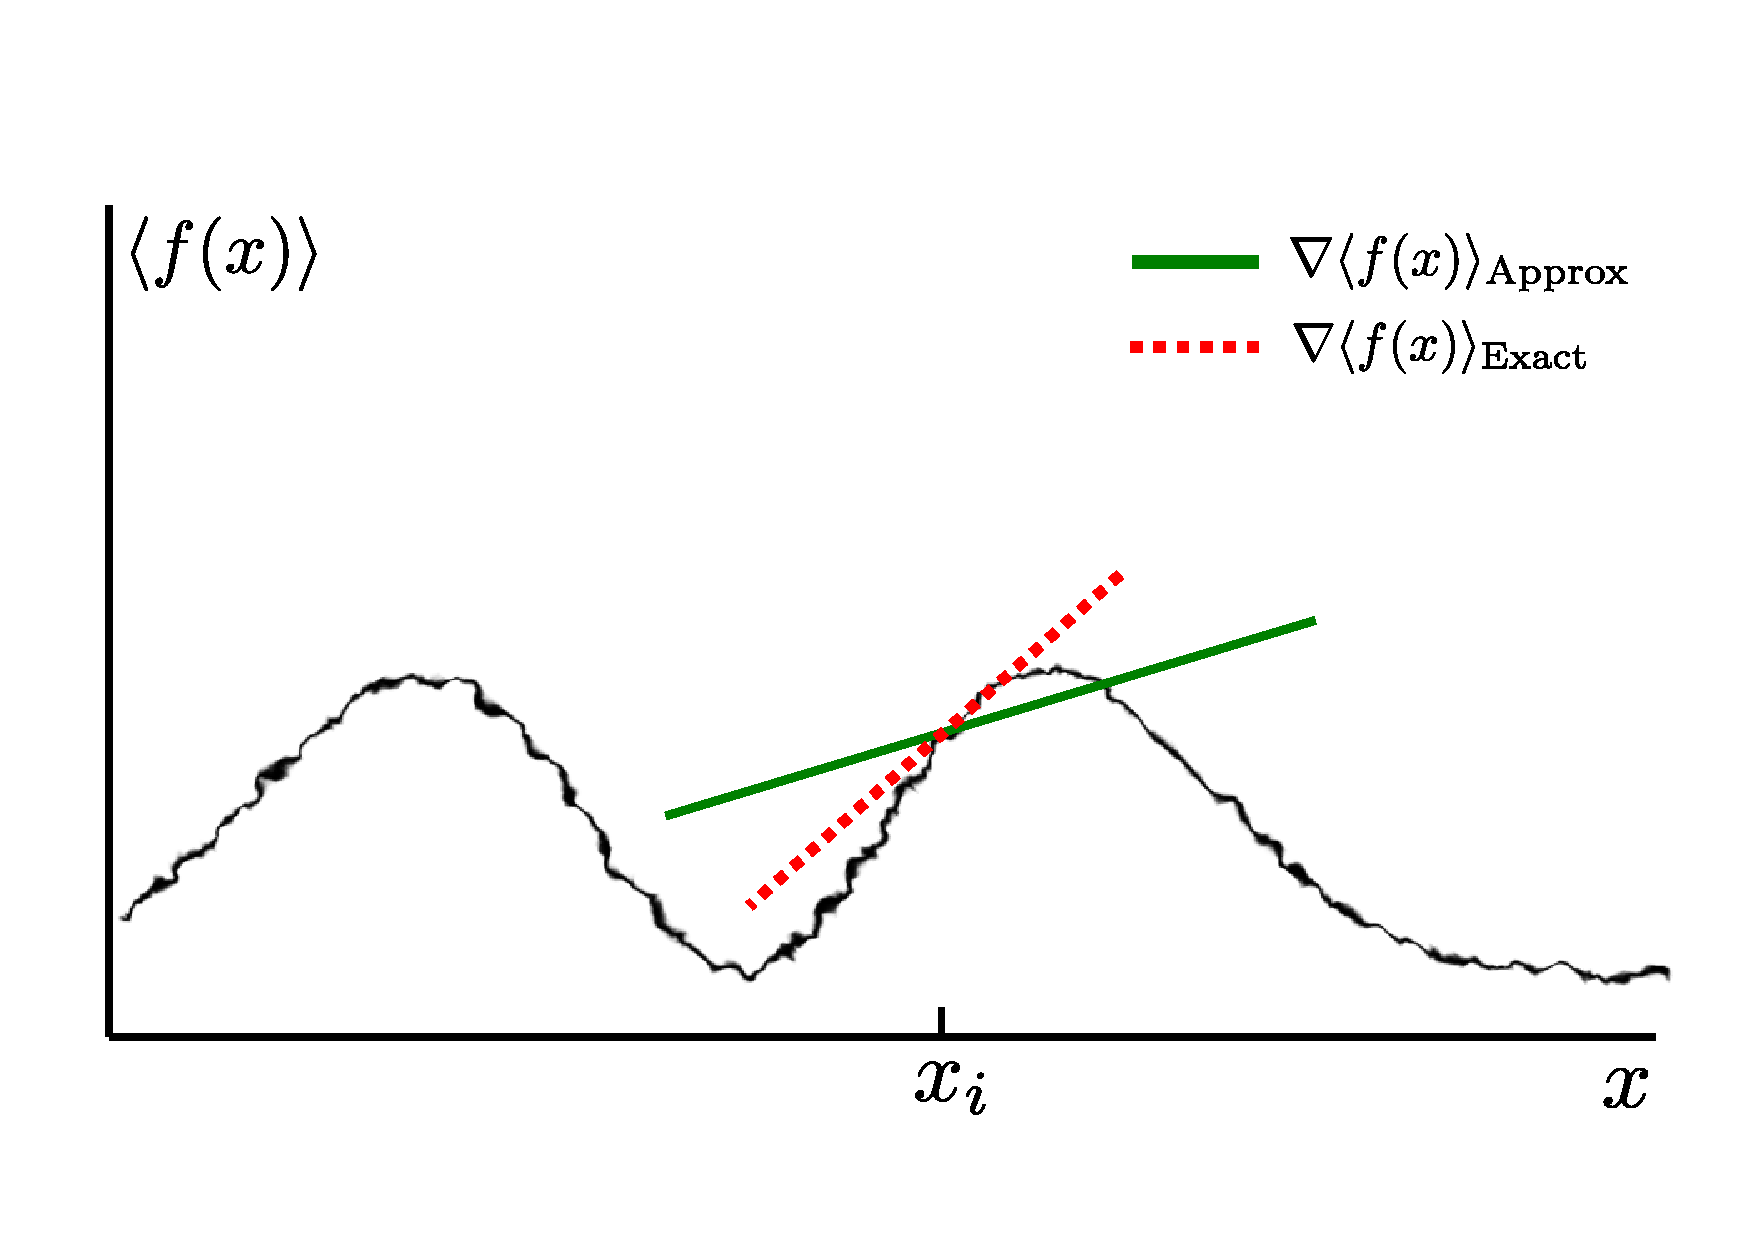
\includegraphics[scale=0.3]{../Graphics/SSGD.pdf}
  \caption{A one dimensional plot of an expectation valued function. Smeared lines are representing uncertainties due to rough sampling. The direction of the local gradient (solid green line) at a point $x_i$ is not necessarily a good estimate of the actual analytic gradient (dashed red line).}
  \label{fig:sSGD}
 \end{center}
\end{figure}


\subsection{Adaptive Stochastic Gradient Descent}

Adaptive Stochastic Gradient Descent (ASGD) has it's roots in the mathematics of automated control theory \cite{ASGD_MB}. The automated process is that of choosing an optimal step length $\delta_i$ for the current transition $x_{i}\to x_{i+1}$. This process is based on the inner product of the old and the new gradient though a variable $X_i$

\begin{equation}
\label{eq:ASGD_X_i}
 X_i \equiv -\nabla_i\cdot \nabla_{i-1}
\end{equation}

The step length from Eq.~(\ref{eq:SGD}) is modeled in the following manner in ASGD

\begin{eqnarray}
 \delta_i   &=& \gamma(t_i) \\
 \gamma(t)  &=& a/(t + A) \label{eq:ASGD_delta_i}\\
 t_{i+1}    &=& \max(t_i + f(X_i), 0) \label{eq:ASGD_t_i}\\
 f(x)       &=& f_\mathrm{min} + \frac{f_\mathrm{max} - f_\mathrm{min}}{1 - (f_\mathrm{max}/f_\mathrm{min})e^{-x/\omega}}\label{eq:ASGD_f_i}
\end{eqnarray}

with $f_\mathrm{max} > 0$, $f_\mathrm{min} < 0$, and $\omega > 0$. Free parameters are $a$, $A$ and $t_0$, however, Ref. \cite{ASGD} suggests $A=20$ and $t_0=t_1=A$ for universal usage.

Notice that the step length increase if $t_i$ decrease and vice-versa. A smaller step length is sought for regions close to the minimum. The function $f(x)$ is responsible of altering the step length by changing the trend of $t$. Close to the minimum, a smaller step length is sought, and hence $t$ must increase. Being close to the minimum implies that the gradient changes sign frequently. Crossing the minimum with ASGD has the following consequence

\begin{itemize}
 \item Eq.~(\ref{eq:ASGD_X_i}): The value of $X_i$ will be positive.
 \item Eq.~(\ref{eq:ASGD_f_i}): $f(X_i)$ will return a value in $[0, f_\mathrm{max}]$ depending on the magnitude of $X_i$.
 \item Eq.~(\ref{eq:ASGD_t_i}): The value of $t$ will increase, i.e. $t_{i+1} > t_i$.
 \item Eq.~(\ref{eq:ASGD_delta_i}): The step length will decrease.
\end{itemize}

The second step regarding $f(X_i)$ can be visualized in Fig. \ref{fig:f_ASGD}.

\begin{figure}
 \begin{center}
  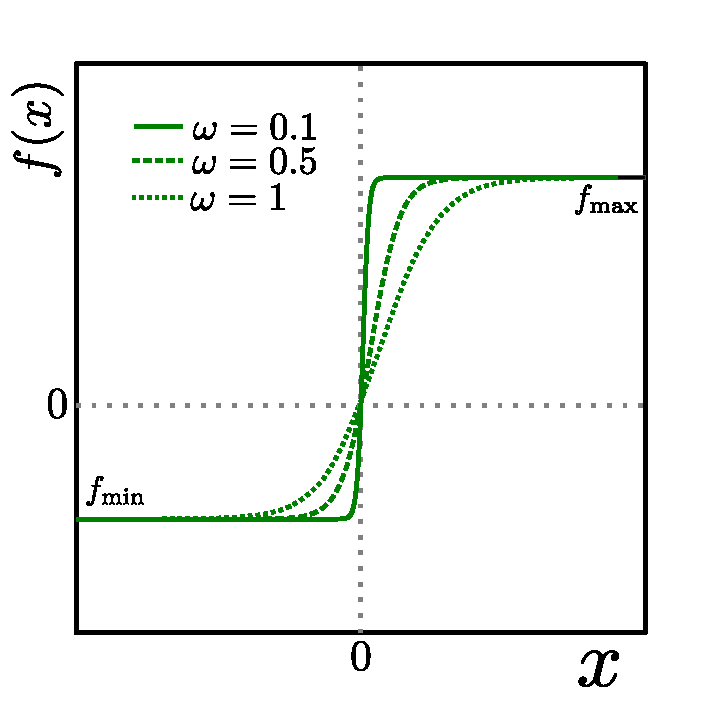
\includegraphics[scale=0.75]{../Graphics/ASGD_f.pdf}
  \caption{Examples of $f(X_i)$ as published in ref. \cite{ASGD}. As $\omega\to0$, $f(x)$ approaches a step function.}
  \label{fig:f_ASGD}
 \end{center}
\end{figure}

\subsubsection{Assumptions}

These assumptions are selected direct citations from Ref. \cite{ASGD}. They are listed in order to give an impression that the shapes of the functions used in ASGD are not selected at random, but carefully chosen to work optimally in a stochastic space with estimated averages involving very few samples.

\begin{itemize}
 \item The statistical error in the sampled gradients are distributed with zero mean.
\end{itemize}

This is shown in ref. to be true; they are normally distributed. The implication is that upon combining gradient estimates for $N$ different processes, the accumulative error will tend to zero quickly.

\begin{itemize}
 \item The step length $\gamma(t)$ is a positive monotone decreasing function defined on $[0,\infty)$ with maximum at $t=0$.
\end{itemize}

With $\gamma(t)$ being as in Eq~(\ref{eq:ASGD_delta_i}), this is easily shown.

\begin{itemize}
 \item The function $f(x)$ is continuous and monotone increasing with $f_\mathrm{min} = \displaystyle\lim_{x\to\infty} f(x)$ and $f_\mathrm{max} =  \displaystyle\lim_{x\to-\infty} f(x)$.
\end{itemize}

This is exactly the behavior displayed in Fig. \ref{fig:f_ASGD}.

\subsubsection{Implementation}

A flow chart of the implementation is given in Fig. \ref{fig:ASGD_flow}. For specific details regarding the implementation, see the code \cite{libBorealisCode}. An example of minimization using ASGD is given in Fig. \ref{fig:ASGD_Ex}. 

\begin{figure}[h]
 \begin{center}
  \subfigure{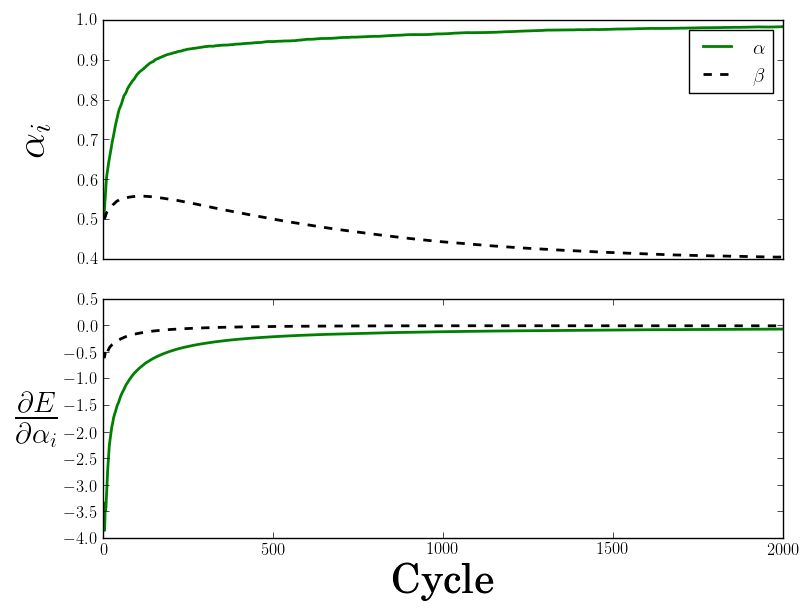
\includegraphics[scale=0.37]{../Graphics/ASGD_min_paramGrad_ex.png}}
  \subfigure{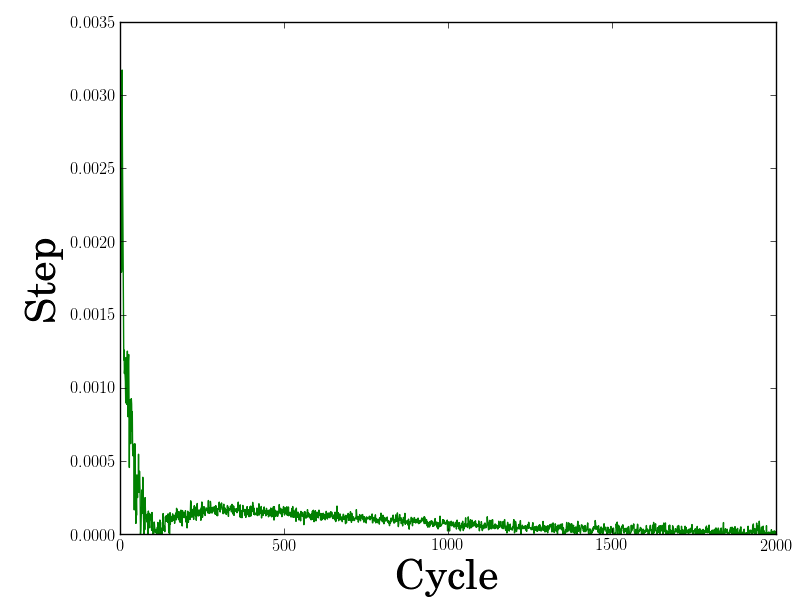
\includegraphics[scale=0.37]{../Graphics/ASGD_min_step_ex.png}} 
  \caption{Results of Adaptive Stochastic Gradient Descent used on a two-particle quantum dot with unit oscillator frequency using $400$ cycles pr. gradient sampling and $40$ independent walkers. The right figure shows the evolution of the time step. The left figure shows the evolution of the variational parameters $\alpha$ and $\beta$ introduced in Section \ref{sec:trialWF} on top, and the evolution of the gradients on the bottom. The gradients are averaged to reveal the pattern underlying the noise. Dispite this averaging, it is apparent that they tend to zero, $\beta$ somewhat before $\alpha$. The step rushes to zero with a small rebound in  as it attempts to cross to negative values.}
  \label{fig:ASGD_Ex}
 \end{center}
\end{figure}


\begin{figure}
 \begin{center}
  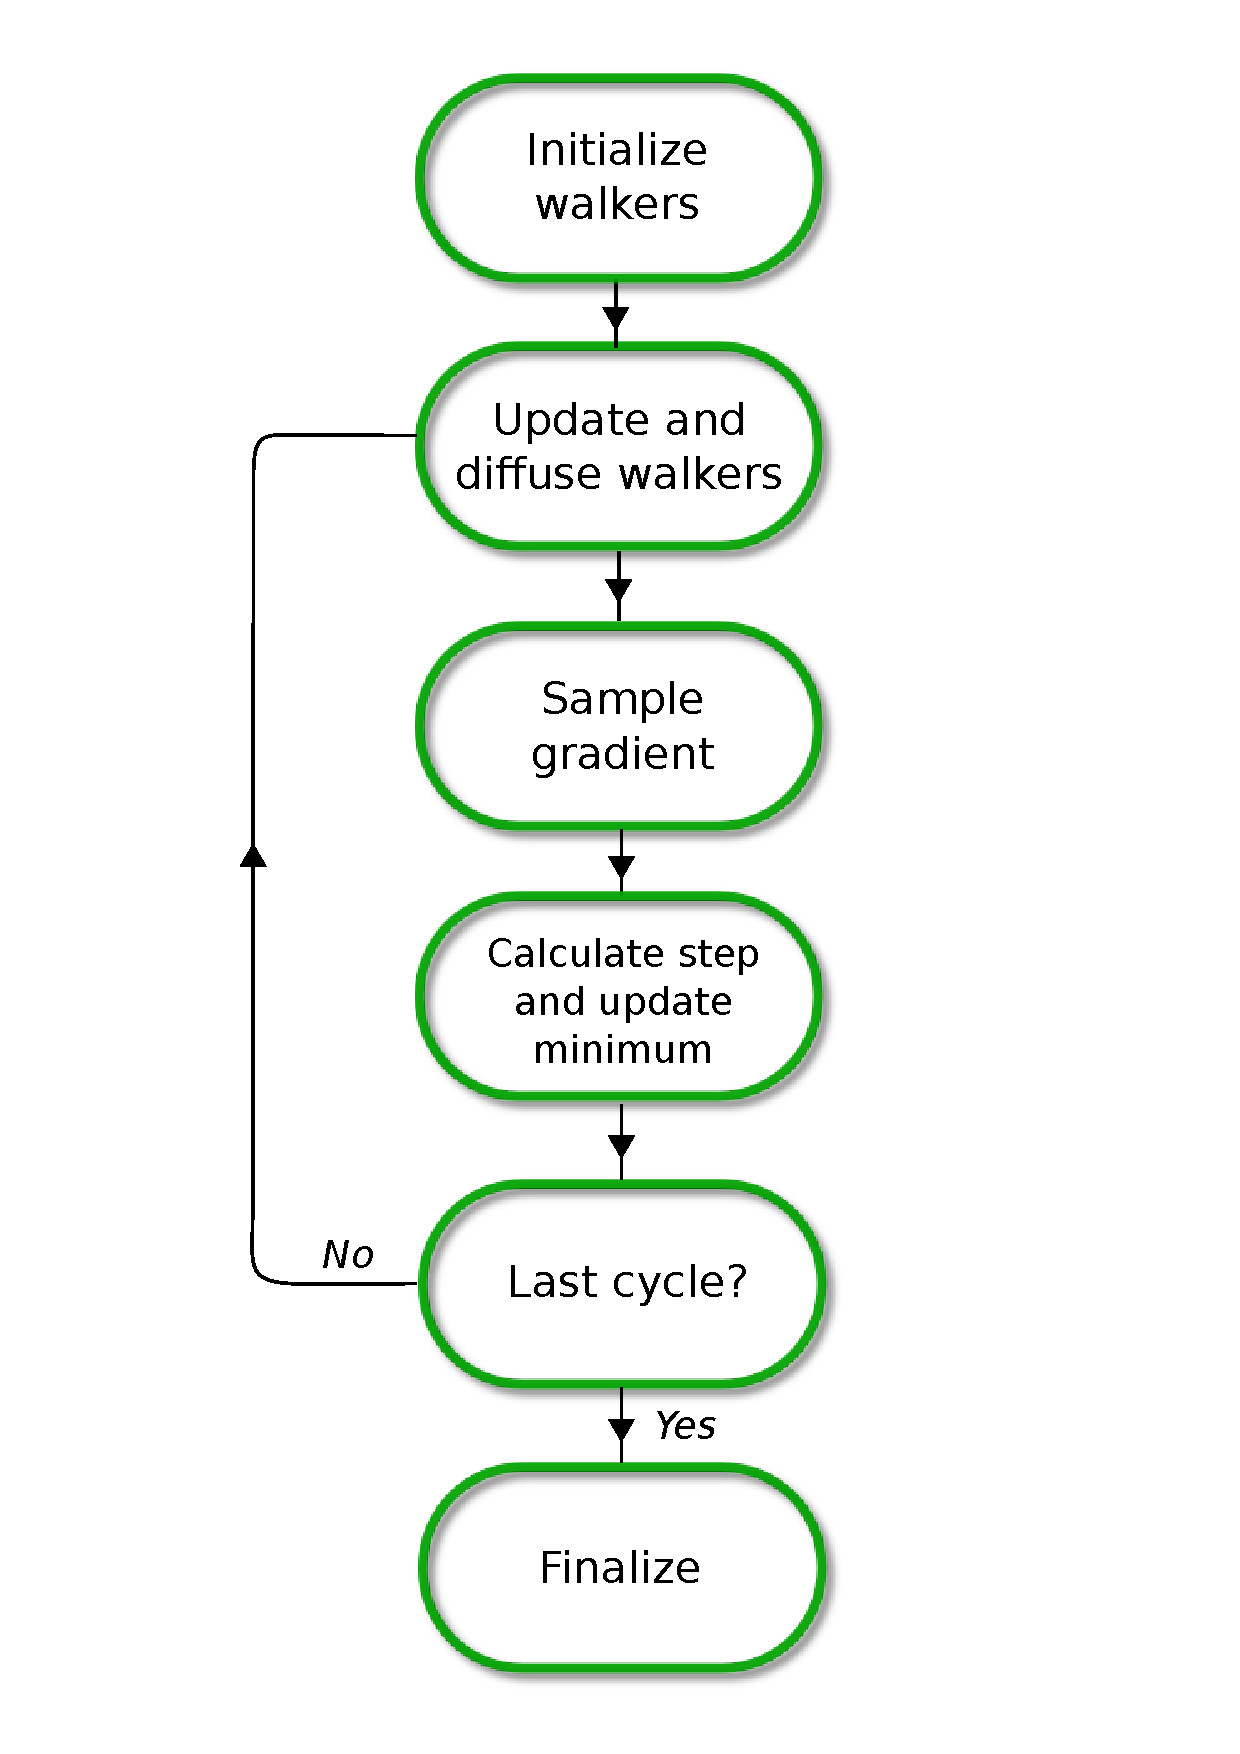
\includegraphics[scale=0.65]{../Graphics/ASGD_UML.pdf}
  \caption{Chart flow of ASGD algorithm. Diffusing a walker is done as described in Fig. \ref{fig:diffFlowChart}. Updating the walkers involves recalculating any values afflicted by updating the minimum. The step is calculated by Eq.~(\ref{eq:ASGD_delta_i}). In case of Quantum Monte-Carlo, the gradient is sampled by Eq.~(\ref{eq:varParGrad}).}
  \label{fig:ASGD_flow}
 \end{center}
\end{figure}
\clearpage


\section{Variational Monte-Carlo}
\label{sec:VMC}

As briefly mentioned in the derivation of the Quantum Monte-Carlo projection process, neglecting the branching term, i.e. set $G_\mathrm{B}=1$, leaves us with a method called Variational Monte-Carlo (VMC). The naming is due to the fact that the method is variational; it supplies as upper bound for the exact ground state energy (see Section \ref{sec:selectingOptVarPar}): The better the trial wave function, the closer the answer is to the exact ground state energy.

Without the branching term, the optimal converged state of the Markov Chain is to span that of the trial wave function. From the flow chart of the VMC algorithm in Fig. \ref{fig:VMCchart}, it is clear that VMC corresponds to nothing but a standard Monte-Carlo integration of the local energy, distributing the points according to the trial wave function (ensured by the Metropolis algorithm and the Langevin equation).

\subsection{Motivating the use of Diffusion Theory}

The question becomes: Why bother with all the diffusion theory if the result is simply an expectation value? Statistics states that \textit{any} distribution may be used when calculating an expectation value. Why bother with a trial wave function, thermalization, and so on? 

The reason is simple, yet not obvious. The quantity of interest, the local energy, is \textit{wave function dependent} $\PT$. Eq.~(\ref{eq:VMCrandomDistE} implies that the evaluation of the local energy in an arbitrary distribution $P(\mathbf{r})$ is \textit{undefined} at the zeros of $\PT$, a ``$0/0$'' expression:

\begin{eqnarray}
 E_\mathrm{VMC} &=& \int P(\mathbf{r}) \frac{1}{\PT}\OP{H}\PT\mathrm{d}\mathbf{r} \nonumber\\
                   &\simeq& \frac{1}{n}\sum_{i=1}^n \frac{1}{\Psi_T(\mbf{r}_i)}\OP{H}\Psi_T(\mbf{r}_i), \label{eq:VMCrandomDistE}
\end{eqnarray}

where the points $\mbf{r}_i$ are drawn from the distribution $P(\mathbf{r})$.

The important fact is that the integral \textit{needs} to importance sampled with the distribution $P(\mathbf{r})=|\PT|^2$  in order to solve the integral in a satisfying manner, that is, avoid sampling close to the roots of $\PT$ without ``cheating''. Introducing importance sampling is done by simply switching distributions (since the calculated value of interest is an expectation value, there is no need to scale the sampled function as is done for standard arbitrary integrals).

Suggesting new positions (diffusion) boils down to be analogous to calling a \textit{random number generator} corresponding to the trial wave function squared distribution. The problem was the roots of $\PT$, however, the distribution of points now share these roots, i.e. the probability of sampling a point where the local energy is undefined equals zero. 

\begin{equation}
 \Psi_T(x_m) = 0 \quad\Longrightarrow\quad P(x_m) = 0
\end{equation}

In other words, the more undefined the energy is at a point, the less probable the point is. This hidden detail is what  Quantum Monte-Carlo safely takes care of that standard Monte-Carlo does not. 

\begin{figure}
 \begin{center}
  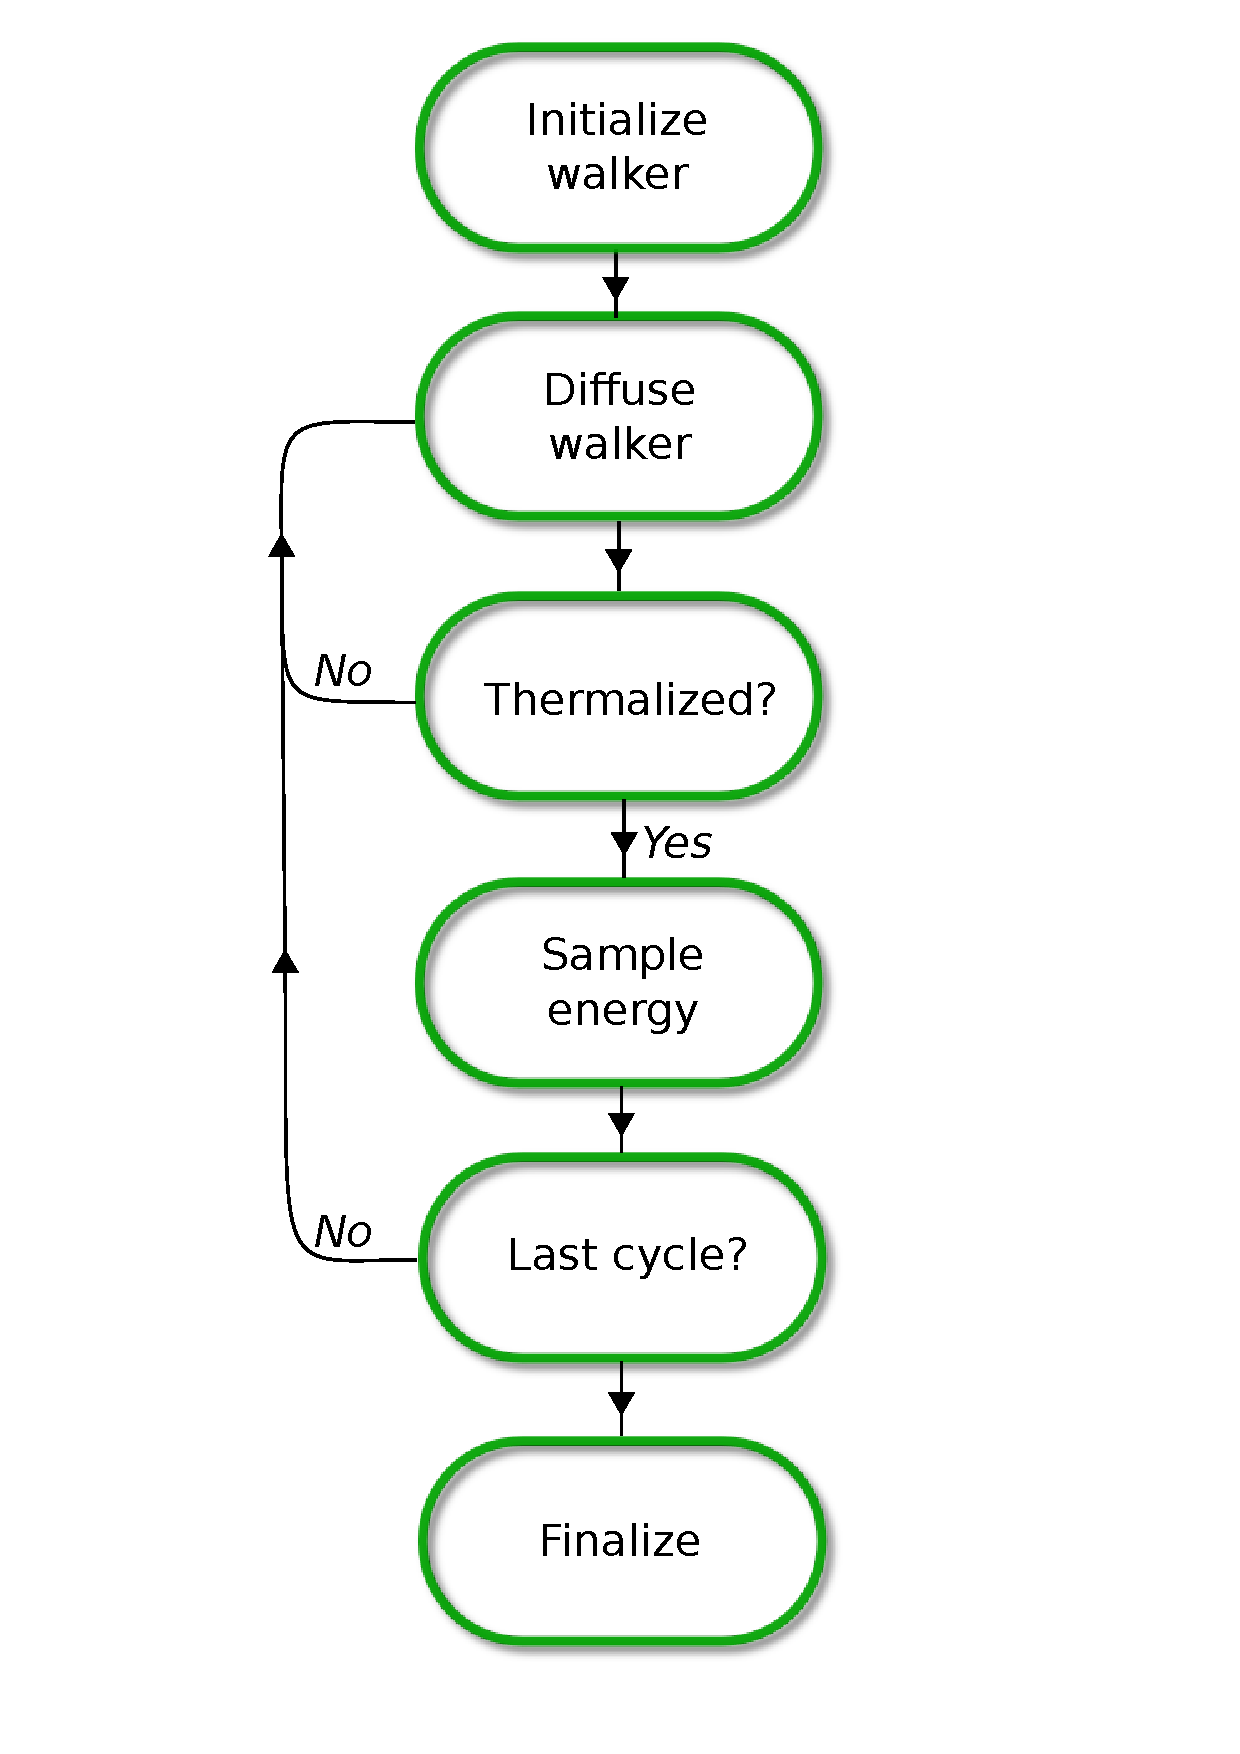
\includegraphics[scale=0.65]{../Graphics/VMCUML.pdf}
  \caption{Chart flow of the Variational Monte-Carlo algorithm. The second step, \textit{Diffuse Walker}, is the process described in Fig. \ref{fig:diffFlowChart}. Energies are sampled as described in Section \ref{sec:calcExpVals}. Thermalization is usually set to a fixed number of cycles. }
  \label{fig:VMCchart}
 \end{center}
\end{figure}
\clearpage

\subsection{Implementation}

Variational Monte-Carlo does not benefit much from an increase of samples (beyond a given point, that is). It is much more important that the system is thermalized, than that the number of walkers are high, or the final amount of samples are huge. It is therefore sufficient to use a single walker pr. VMC process.

The single walker is initialized in a normal distributed manner (with variance $2D\delta\tau$), and released to diffuse according to the process in Fig. \ref{fig:diffFlowChart}. A flow chart of the VMC algorithm is given in Fig. \ref{fig:VMCchart}. Finalizing the sampling involves scaling energies, calculating the variance, etc. 

For more details regarding the specific implementation, see the code in ref. \cite{libBorealisCode}.

\subsection{Limitations}

The only limitation in VMC is the choice of trial wave function. This makes VMC extremely robust; it will \textit{always} produce a result. As the overlap $C_0$ in Eq.~(\ref{eq:schrodGeneralSolution2}) approach unity, the VMC energy approaches the exact ground state energy as a monotone decreasing function. Fig. \ref{fig:VMC_wfcomp} described this effect.

\begin{figure}
 \begin{center}
  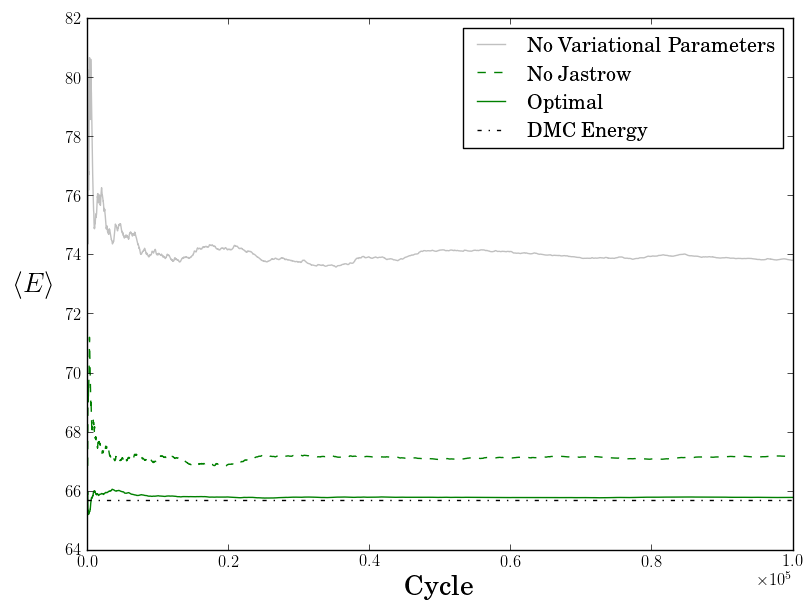
\includegraphics[scale=0.65]{../Graphics/WFComp.png}
  \caption{Comparison of the VMC energy using different trial wave functions. The DMC energy is believed to be very close to the exact ground state. It is apparent that adding a variational parameter to the trial wave function lowers the energy substantially, however, when adding the Jastrow factor (denoted \textit{Optimal}) described in Section \ref{sec:ChoiceTrialWF} the VMC energy gets very close to the ``exact'' answer. Lower energy means a better energy when dealing with variational methods. In this example, a 12 particle quantum dot with unit frequency is used.}
  \label{fig:VMC_wfcomp}
 \end{center}
\end{figure}

\section{Diffusion Monte-Carlo}
\label{sec:DMC}

Applying the full diffusion framework introduced in the previous sections results in a method known as Diffusion Monte-Carlo (DMC)\footnote{In literature, DMC is also known as \textit{Projection Monte-Carlo}, for reasons described in Section \ref{sec:statingDiff}.}. Diffusion Monte-Carlo results are often referred to as \textit{exact}, in the sense that it is overall one of the most precise many-body methods. However, just as any many-body method, DMC also has its limitations. These will be discussed in Section \ref{sec:DMClimitations}.

Where other many-body methods run into the \textit{curse of dimensionality} (CPU-time exponentially increasing with number of particles, precision, etc.), DMC with it's position basis Quantum Monte-Carlo formalism does not. With DMC, it is simply a matter of evaluating a more complicated trial wave function, or simulating for a longer period of cycles, in order to reach convergence to the believed ``exact'' ground state in a satisfactory way.

Details regarding the exactness of DMC will be covered in the section on limitations.

\subsection{Implementation}

DMC is as mentioned a precise method; more statistics is like water in a desert - there is never enough of it. In addition, branching is a major part of the algorithm. In other words: DMC uses a large ensemble of walkers to generate enormous amounts of statistics. These walkers are initialized using a VMC calculation, i.e. the walkers are distributed according to the trial wave function at $\tau=0$. 

There are three layers of loops in the DMC method implemented in this thesis, two of which are obvious: The time-step - and walker loops. However, introducing a third \textit{block loop} within the walker loop boosts the convergence dramatically. This loop continues until the current walker is either dead ($G_B = 0$), or diffused $n_b$ times. Using this method, ``good'' walkers will have multiple offspring pr cycle, while ``bad'' walkers will rarely survive the block loop. Perfect walkers will supply a ton of statistics as they surf through all the loops without branching ($G_B \sim 1$).

A flow chart of the DMC algorithm is given in Fig. \ref{fig:DMCchart}. 

\subsection{Sampling the Energy}

Unlike VMC, DMC does not weigh all walkers equally. It is therefore necessary to weigh each walker's contribution to a cumulative energy sampling accordingly, that is, with the branching Green's function. Let $E_k$ denote the cumulative energy for time-step $\tau = k\delta\tau$, $n_w$ be the number of walkers in our system at time-step $k$, $\tilde n_{b,i}$ be the number of blocks walker $i$ survives, and let $W_i(\vec r, \tau)$ represent walker $i$. The relation is then

\begin{equation}
 E_k = \frac{1}{n_w}\sum_{i=1}^{n_w} \frac{1}{\tilde n_{b,i}}\sum_{l=1}^{\tilde n_{b,i}} G_\mathrm{B}\Big(W_i(\vec r, \tau_k + l\delta\tau)\Big)E_L\Big(W_i(\vec r, \tau_k + l\delta\tau)\Big)
\end{equation}

As the formalism required, setting $G_B = n_w = n_b = 1$ reproduce the VMC algorithm. 

The new trial energy (remember Eq.~(\ref{eq:firstTrialEnergyIntro})) is set to be equal to the previous cycle's average energy  

\begin{equation}
 E_T = E_k
\end{equation}

The DMC energy is updated each cycle to be the trailing average of the trial energies

\cfbox{2.5cm-10pt}{
\begin{equation}
 E_\mathrm{DMC} = \overline{E_T} = \frac{1}{n}\sum_{k=1}^n E_k
\end{equation}
}




\subsection{Limitations}
\label{sec:DMClimitations}

By introducing the branching term, DMC is a far less robust method compared to VMC. Action must be taken in order to stabilize the iterations through tuning of parameters such as population size, time-step, block size, etc. This is the disadvantage of DMC compared to other many-body methods such as Coupled Cluster, which is far more automatic.

\subsubsection{Time Step Errors}

The error introduced by the short time approximation goes as $\mathcal{O}(\delta\tau^2)$ (see Eq.~(\ref{eq:shortTimeApprox})). There is a second error related to the time-step, arising from the fact that not all steps are accepted by the Metropolis algorithm. This introduces a effective reduction in the time step, and is countered by scaling the time step with the acceptance ratio upon calculating $G_B$. However, DMC is rarely used without importance sampling (Fokker-Planck), which, due to the Quantum Force, has an acceptance ratio $\sim 1$. It is therefore common to ignore this problem, and use a sufficiently low time step.

\subsubsection{Selecting the Time-step}

Studying the branching Green's function in equation \ref{eq:branchFP} in more detail reveals that it's magnitude increase exponentially with the spread of the energies

\begin{equation}
G_B \propto \exp{\left(\Delta E\delta\tau\right)} 
\end{equation}

As will be shown in Section \ref{sec:varAndSTD}, the spread in energy samples are higher the worse of an approximation to the ground state the trial wave function is. In addition, the magnitude of the spread scales with the magnitude of the energy. Due to finite computer memory, $N$ slots in the memory are dedicated for storing walkers on every node. Too large branching factors may cause the system to max out the memory on one node before the walkers can be redistributed across all the nodes. 

Setting an upper bound to the branching might seem like a good idea, however, with these fluctuations, this would imply an imbalance in the population drift, causing the walkers to slowly die out or reach a state not representing the desired projection.

The solution is to balance out the increase in $\Delta E$ by lowering the time-step accordingly. However, too low a time-step will hinder DMC to evolve walkers efficiently, especially if the positional span of the distribution is large. If the walkers are inefficient, that is, the trial energy converges slowly, the projection process will be equally slow. This has been verified by calculations in this thesis; slowly converging systems, such as low frequency quantum dots, will have densities which look far from the radially symmetric expected result if the time step or the number of walkers (the amount of statistics) is too low.

Another source of error is due to the \textit{fixed node approximation}. This approximation will be covered in the next section.

\begin{figure}[ht]
 \begin{center}
  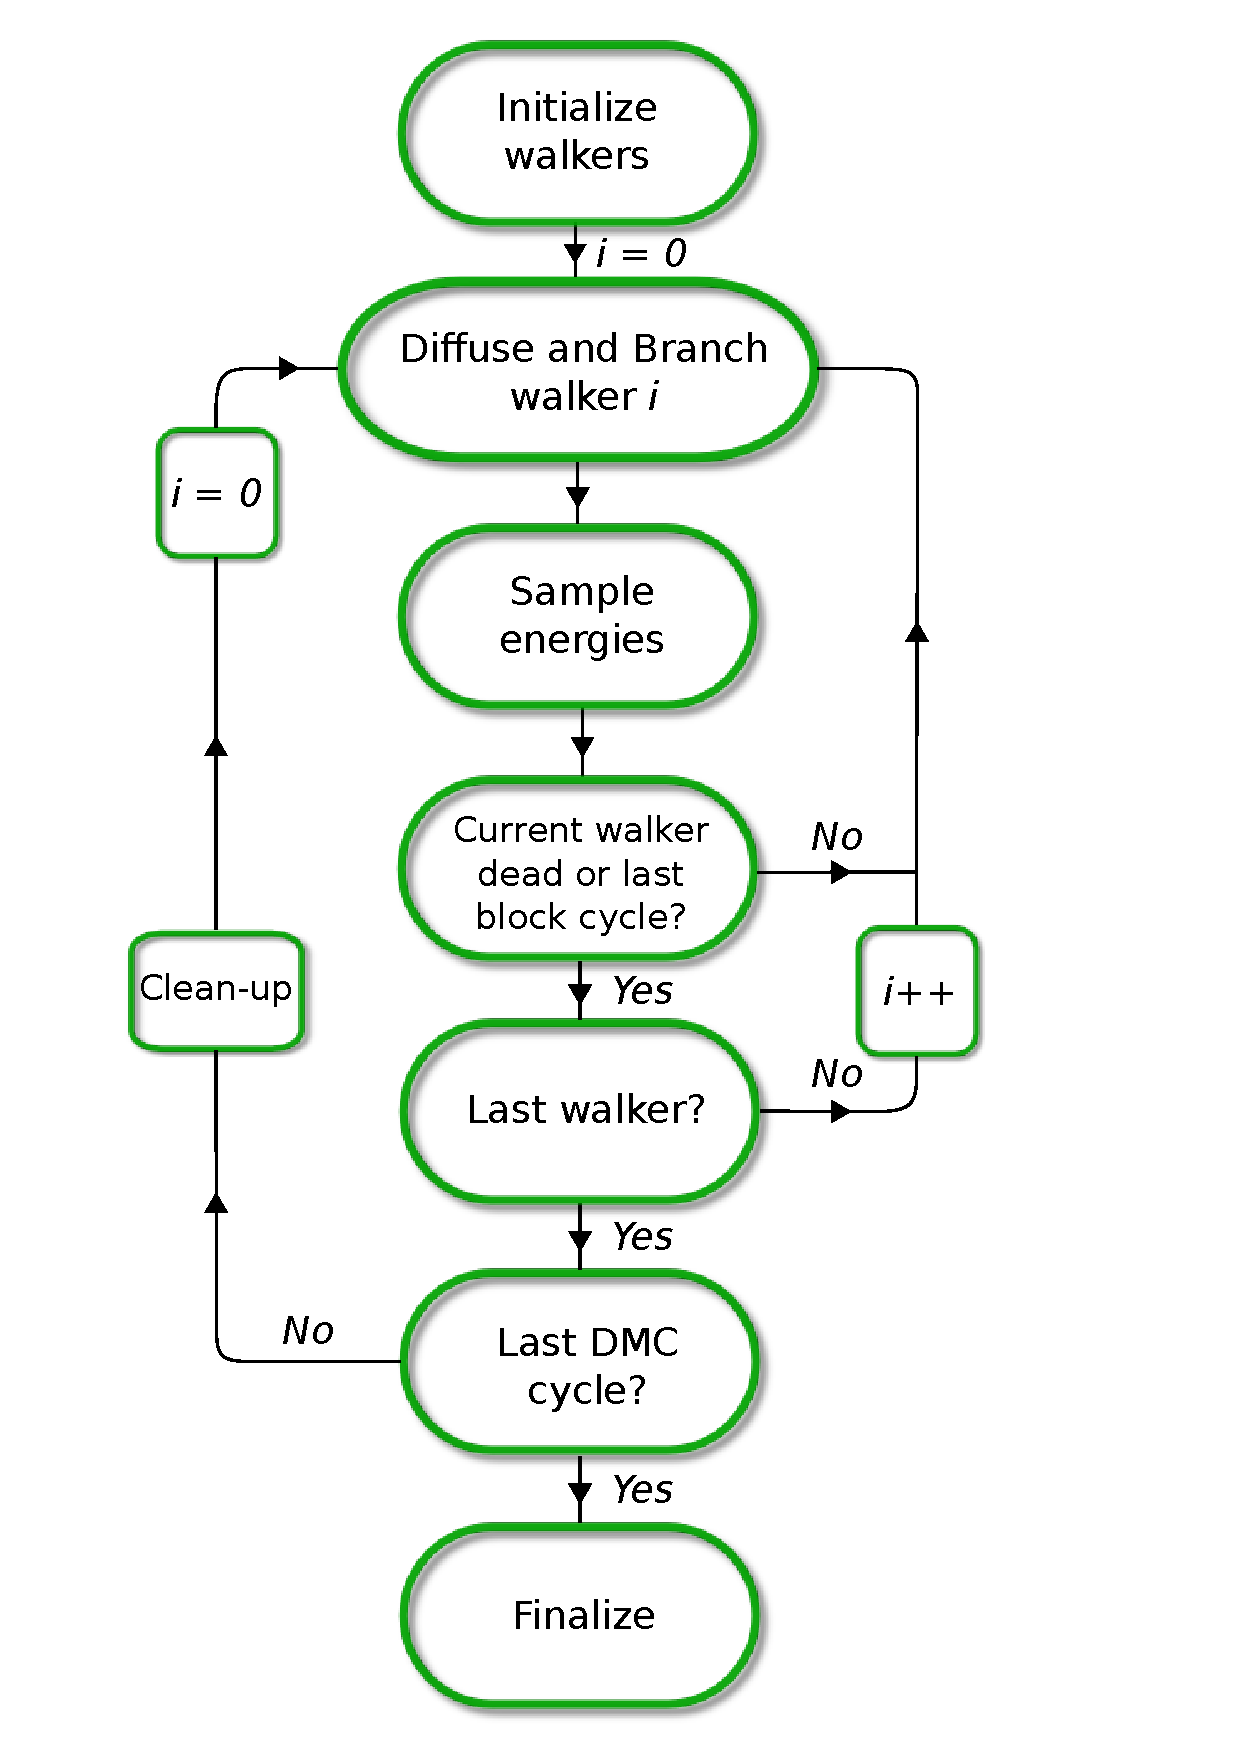
\includegraphics[scale=0.65]{../Graphics/DMCUML.pdf}
  \caption{Chart flow of the Diffusion Monte-Carlo algorithm. The count variable \textit{i} is the index of the walker loop. The second step, \textit{Diffuse and Branch Walker}, is the process described in Fig. \ref{fig:diffFlowChart} in combination with the branching from Fig. \ref{fig:branching}. Energies are sampled as described in Section \ref{sec:DMC}. Thermalization is not done in the same way as VMC (see Fig. \ref{fig:VMCchart}), but rather includes the entire flow with a reduced number of DMC - and block cycles.}
  \label{fig:DMCchart}
 \end{center}
\end{figure}
\clearpage

\subsection{Fixed node approximation}

Looking at Eq.~(\ref{eq:BosonicWFExplicit}), it is apparent that by choosing positive phases for the single particle wave functions, the bosonic many-body wave function is exclusively positive. For fermions however, the sign change upon interchange of two particles introduce the possibility that the wave function will have both negative and positive regions, independent of the choice of phases in the single particle wave functions.

As importance sampled DMC iterates, the density of walkers at a given time, $P(x, \tau)$, represents the projected wave function from Eq.~(\ref{eq:schrodGeneralSolution2}) multiplied by the trial wave function (see the end of Section \ref{sec:anisFokker} for details)

\begin{equation}
 P(\mathbf{r}, \tau) = \Ptau\PT,
\end{equation}

where theoretically using an exact projection operator

\begin{equation}
  \lim_{\tau\to\infty} P(\mathbf{r}, \tau) = \braket{\Phi_0}{\Phi_T}\Phi_0(\mathbf{r})\Psi_T(\mathbf{r}),
\end{equation}

which, if interpreted as a density, should always be greater than zero. In the case of fermions, this is not guaranteed, as
the node structure, i.e. the roots, of the exact ground state and the trial wave function will generally be different.  

To avoid this anomaly in the density, $\Ptau$ and $\PT$ have to change sign simultaneously\footnote{It should be mentioned that more sophisticated methods exist for dealing with the sign problem, some of which splits the distribution of walkers into a negative and a positive regions, however, due to the infinity position space, this requires an enormous amount of walkers to succeed.}. The brute force way of solving this problem is to \textit{fix} the nodes by rejecting a walker's step if the trial wave function changes sign:

\begin{equation}
\frac{\Psi_T(\mathbf{r}_i)}{\Psi_T(\mathbf{r}_j)} < 0 \quad\Longrightarrow\quad A(i\,\rightarrow\,j) = 0
\end{equation}

where $A(i\,\rightarrow\,j)$ is the probability of accepting the move, as described in Section \ref{sec:MetroMain}. An illustrative example is attempted in Fig. \ref{fig:fixxednode}.

\begin{figure}
 \begin{center}
  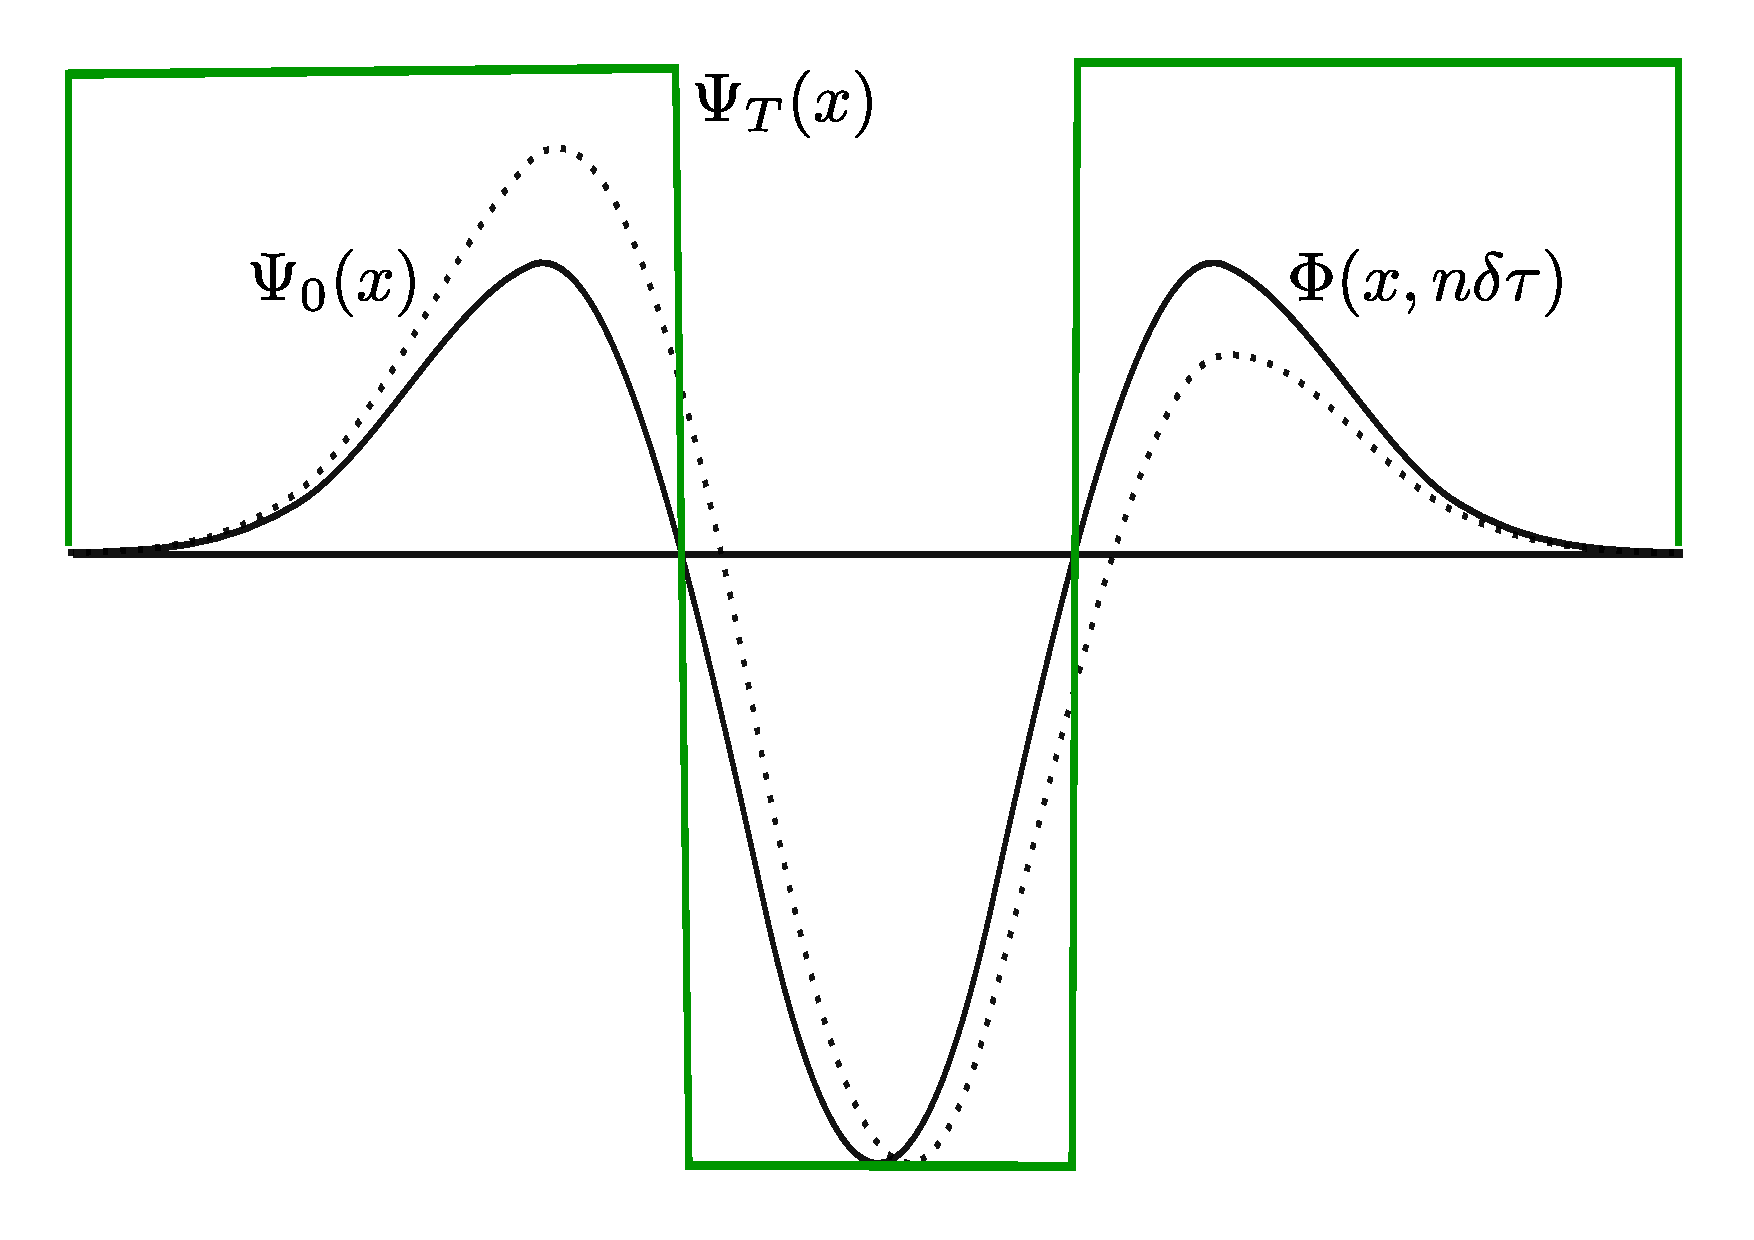
\includegraphics[scale=0.3]{../Graphics/fixxednode.pdf}
  \caption{A one-dimensional illustration of the fixed node approximation. The dotted line is the exact ground state $\Psi_0(x)$. The distribution of walkers at cycle $n$, $\Phi(x, n\delta\tau)$, similar in shape with $\Psi_0(x)$, however, sharing nodes with the trial wave function $\Psi_T(x)$ (box-like function for illustration purposes), and thus making it impossible to match the true ground state exactly.}
  \label{fig:fixxednode}
 \end{center}
\end{figure}


\section{Estimating One-body Densities}
\label{sec:OBD}

The one-body density is defined as

\begin{equation}
 \rho(  \mathbf{r}_1) = \iint\limits_{  \mathbf{r}_2   \mathbf{r}_3}...\int\limits_{  \mathbf{r}_N} \left|\Phi(  \mathbf{r}_1   \mathbf{r}_2 ...   \mathbf{r}_N)\right|^2\mathrm{d}  \mathbf{r}_2...\mathrm{d}  \mathbf{r}_N.
\end{equation}

Unlike the distribution $|\Phi(\mathbf{r})|^2$, which describes the distribution of any of the particles in the system, the one-body density $\rho(\mathbf{r}_1)$ describes the simultaneous distribution of every particle in the system, that is, $\rho(\mathbf{r}_1)\mathrm{d}\mathbf{r}_1$ represents the probability to find \textit{any} of the systems $N$ particles within the volume element $\mathrm{d}\mathbf{r}_1$. Due to the indistinguishable nature of the particles, the fact that the first coordinate is chosen is purely conventional; any of the $N$ coordinates contain information about all the particles. For the same reason, the one-body density should be normalized to the number of particles $N$, and not unity.   

The one-body density integral corresponds to projecting every degree of freedom into one. In a Monte-Carlo simulation, estimating this quantity is done by collecting snapshots of the walkers' positions. These snapshots serve as samples to a histogram where each set of Cartesian coordinates (independent of particle number) give rise to one histogram-count ($\mathrm{d}\mathbf{r}_1$ is approximated by a finite value).

\subsection{Estimating the Exact Ground State Density}

The one-body density of the trial wave functions is in other words trivial; create a histogram of sampled VMC positions. The challenge is estimating the one-body density of the exact wave function, given a set of DMC data. As described in Section \ref{sec:anisFokker}, the distribution of walkers by design spanning the \textit{mixed density} $f(\mathbf{r}, \tau) = \Ptau\PT$, which does not correspond to the ground state distribution unless the trial wave function is indeed the exact ground state. 

This implies the need of a method to transform the one-body density of $f(\mathbf{r}, \tau)$) into the one of $|\Ptau|^2$ (from here on referred to as the \textit{pure density}). This is done by using a third estimate obtained from VMC, the \textit{variational density}, which corresponds to the one-body density of $|\Psi_T(\mathbf{r})|^2$. To achieve this, a relation shown in in Ref. \cite{abInitioMC} by Taylor expanding $\bra{\Phi_0}\OP{A}\ket{\Phi_0}/\braket{\Phi_0}{\Phi_0}$ around $\Delta \equiv \PT - \Ptau$ serves as a good starting ground

\begin{align}
 \langle A \rangle_0 = \frac{\bra{\Phi_0}\OP{A}\ket{\Phi_0}}{\braket{\Phi_0}{\Phi_0}} &\simeq  2\frac{\bra{\Phi_0}\OP{A}\ket{\Psi_T}}{\braket{\Phi_0}{\Psi_T}} -  \frac{\bra{\Psi_T}\OP{A}\ket{\Psi_T}}{\braket{\Psi_T}{\Psi_T}} + \mathcal{O}(\Delta^2)\notag\\
  &= 2\langle A \rangle_\mathrm{DMC} - \langle A \rangle_\mathrm{VMC}  + \mathcal{O}(\Delta^2) \label{eq:PureEstimRelat}
\end{align}

Expressed in terms of \textit{density operators} (not one-body densities), the expectation values become

\newcommand{\tr}{\mathrm{tr}}

\begin{align*}
 \langle A \rangle_0 &= \tr(\OP{\rho}_0\OP{A}) \\
 \langle A \rangle_\mathrm{VMC} &= \tr(\OP{\rho}_\mathrm{VMC}\OP{A}) \\
 \langle A \rangle_\mathrm{DMC} &= \tr(\OP{\rho}_\mathrm{DMC}\OP{A}) 
 \end{align*}

where $\tr$ denotes the \textit{trace} (sum of eigenvalues\cite{leinaas}). Inserting these equation into Eq.~(\ref{eq:PureEstimRelat}) yields

\begin{align}
 \tr(\OP{\rho}_0\OP{A}) &\simeq 2\tr(\OP{\rho}_\mathrm{DMC}\OP{A}) -  \tr(\OP{\rho}_\mathrm{VMC}\OP{A}) + \mathcal{O}(\Delta^2) \notag\\
  &\simeq \tr\left(\left(2\OP{\rho}_\mathrm{DMC} - \OP{\rho}_\mathrm{VMC}\right)\OP{A}\right) + \mathcal{O}(\Delta^2)
\end{align}

which leads to the conclusion that the mixed density can be transformed in the following manner

\begin{equation}
 \OP{\rho}_0 \simeq 2\OP{\rho}_\mathrm{DMC} - \OP{\rho}_\mathrm{VMC} \label{eq:densityTransform}
\end{equation}

The transformation of densities into one-body densities can be applied to both sides of this equation, implying that combining the one-body densities of $f(\mathbf{r}, \tau)$ from DMC and the trial wave function one from VMC according to Eq.~(\ref{eq:densityTransform}) serves as a good approximation to the one-body density of the iterated wave function $\Ptau$ given that it is close to the exact wave function.

\subsection{Radial Densities}

In the case of symmetric wave functions, like in the case for atoms and quantum dots, the radial one-body density is obtained by integrating out the angular dependencies of the one-body density. This corresponds to weighing all angular directions equally in a brute for average and can only be applied to radially symmetric systems without loosing information.

Calculating the integral in two and three dimensions yields

\begin{align}
 I_\mathrm{3D} &= \iint \rho (\mathbf{r}_1, \theta_1, \phi_1)r_1^2\sin\theta_1\mathrm{d}\theta_1\mathrm{d}\phi_1 \notag\\
   &\propto r_1^2\rho(\mathbf{r}_1) \label{eq:averagedRadialOBD_3D} \\
 I_\mathrm{2D} &= \int \rho (\mathbf{r}_1, \phi_1)r_1\mathrm{d}\phi_1 \notag\\
   &\propto r_1\rho(\mathbf{r}_1) \label{eq:averagedRadialOBD_2D}
\end{align}

In practice, this integral is calculated by creating a histogram $H(r)$ of all sampled radii. Transforming this histogram into the radial one-body density $\rho(r_1)$ is according to Eq.~(\ref{eq:averagedRadialOBD_3D}) and Eq.~(\ref{eq:averagedRadialOBD_2D}) done in the following manner

\begin{equation}
 \rho(\mathbf{r}_1) = \frac{H(\mathbf{r}_1)}{r_1^{(d-1)}}\label{eq:radial_OBD}
\end{equation}

where $d$ denotes the number of dimensions. An example radial one-body density is given in Fig. \ref{fig:OBD_ex}

\begin{figure}
 \begin{center}
  \subfigure{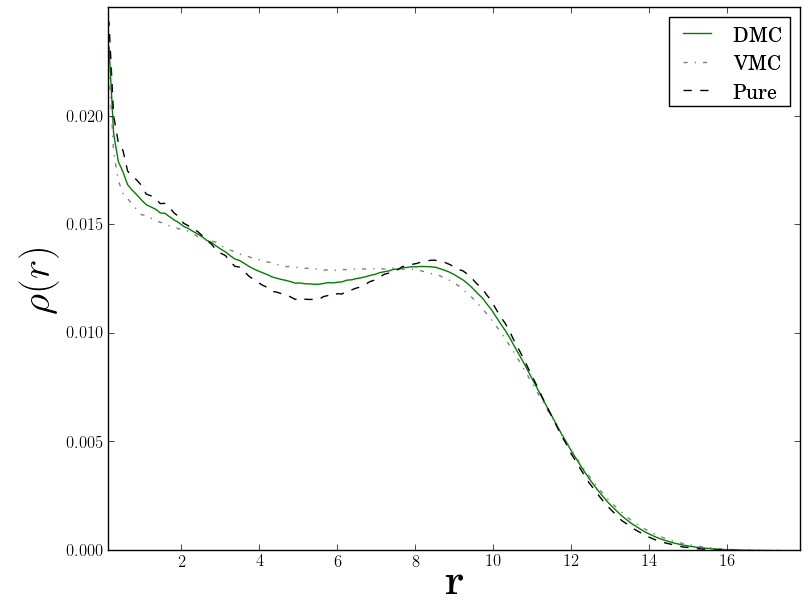
\includegraphics[scale=0.35]{../Graphics/OBD_rad_ex_12pw01.png}}
  \subfigure{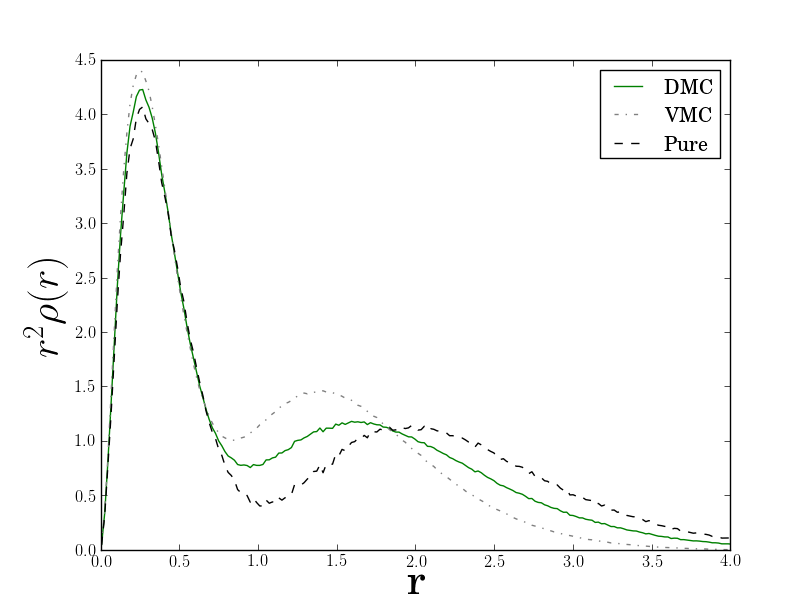
\includegraphics[scale=0.3816]{../Graphics/OBD/OBD_Atoms/2D/Beryllium.png}}
  \caption{Two examples of radial one-body densities for both VMC, DMC (from $f(\mathbf{r}, \tau)$), and the pure density from Eq.~(\ref{eq:densityTransform}). On the left: A 12-particle quantum dot with $\omega=0.1$. The density diverges close to zero due to a ``$\frac{0}{0}$'' expression (see Eq.~(\ref{eq:radial_OBD})). On the right: Unscaled radial density for the beryllium atom, i.e. $r_1^2\rho(\mathbf{r}_1)$. These results will be discussed in the results section.}
  \label{fig:OBD_ex}
 \end{center}
\end{figure}

It should be noted that in the case of atoms, the one-body density does not reveal particularly interesting shapes (this will be presented in Figure \ref{fig:OBD_noble_Atoms_2D_combo}), however, simply showing the distribution of radii, that is, not dividing by $\mathbf{r}_1^2$ reveal interesting shapes which can be used to discuss the physics of different atoms. 



\section{Estimating the Statistical Error}

As with any statistical result, the statistical errors needs to be supplied in order for it to be taken seriously. Systematic errors, that is, errors introduced due to limitations in the model, is discussed in each method's respective section, and will not be related to the statistical error. 

Statistical errors, that is, the  deviation from the true ensemble average due to the fact that the equality in Eq.~(\ref{eq:MeanVStrueExp}) can never be fulfilled, can be estimated using several methods, some of which are \textit{naive} in the sense that they assume the dataset to be completely \textit{uncorrelated}, i.e. the samples are independent of each other.

\subsection{The Variance and Standard Deviates}
\label{sec:varAndSTD}

Given a set of samplings, e.g. local energies, the variance is a measure of their spread from the true mean value

\begin{eqnarray}
\label{eq:variance}
\Var(E) &=& \Exp{(E-\Exp{E})^2} \nonumber\\
        &=& \Exp{E^2} - 2\underbrace{\Exp{E\Exp{E}}}_{\Exp{E}\Exp{E}} + \Exp{E}^2 \nonumber\\
        &=& \Exp{E^2} - \Exp{E}^2 \\
        &\simeq& \overline{E^2} - \overline{E}^2
\end{eqnarray}

In the case of having the exact wave function, i.e $\ket{\Psi_T} = \ket{\Psi_0}$, the variance becomes zero:

\begin{eqnarray*}
\label{eq:varianceZeroExact}
\Var(E)_\mathrm{Exact} &=& \bra{\Psi_0}\OP{H}^2\ket{\Psi_0} -  \bra{\Psi_0}\OP{H}\ket{\Psi_0}^2 \\
		        &=& E_0^2 - (E_0)^2 \\
		        &=& 0
\end{eqnarray*}

The variance is in other words an excellent measure of how good of a fit different trial wave functions are to the system. A common misconception is that the numerical value of the variance can be used to compare properties of \textit{different} systems. For instance, if system $A$ has variance equal to half of system $B$'s, one could easily conclude that system $A$ has the best fitting trial wave function. However, this is not true. The variance has unit energy squared (in the case of local energies), and will thus scale with the magnitude of the energy. One can only safely use the variance as a direct measure locally in each specific system, e.g. Beryllium simulations.

Another misconception is that the variance is a direct numerical measure of the error. This can in no way be true given that the units mismatch. The \textit{standard deviation}, $\sigma$, is the square root of the variance,

\begin{equation}
\label{eq:stdNaive}
 \sigma^2(x) = \Var(x),
\end{equation}


and has hence a unit equal to that of the measured value. It is therefore related to the \textit{spread} in the sampled value; zero deviation implies perfect samples, while increasing deviation means increasing spread and statistical uncertainty. The standard deviation is in other words a useful quantity when it comes to calculating the error, i.e. the expected deviation from the exact mean $\Exp{E}$.

\subsection{The Covariance and correlated samples}

It was briefly mentioned in the introduction that certain error estimation techniques was too naive in case of correlated samples. Two samples, $x$, $y$, are said to be correlated if their \textit{covariance}, $\Cov(x, y)$, is non-zero

\begin{eqnarray}
\label{eq:covariance}
 \Cov(x, y) &\equiv& \Exp{(x - \Exp{x})(y - \Exp{y})} \nonumber\\
            &=& \Exp{xy - x\Exp{y} - \Exp{x}y + \Exp{x}\Exp{y}} \nonumber\\
            &=& \Exp{xy} - \Exp{x\Exp{y}} \underbrace{-\Exp{y\Exp{x}} + \Exp{\Exp{x}\Exp{y}}}_{0} \nonumber\\
            &=& \Exp{xy} - \Exp{x}\Exp{y}.
\end{eqnarray}

Notice that $\Cov(x,x) = \Var(x)$. Using this definition, whether or not the samples are correlated boils down to whether or not $\Exp{xy} = \Exp{x}\Exp{y}$. 

The consequence of ignoring the correlations is a resulting error estimate which is generally less than the true error; correlated samplings are more clustered, i.e. less spread, due to previous samplings' influence on the value of the current sample\footnote{Samples in QMC is obviously correlated due to the nature of the Langevin equation (difference equation).}. Denoting the true standard deviation as $\sigma_c$, the above discussion can be distilled to

\begin{equation}
 \label{eq:trueVsNaiveSTD}
 \sigma_c(x) \ge \sigma(x),
\end{equation}

where $\sigma(x)$ is the deviation from Eq.~(\ref{eq:stdNaive}). 


\subsection{The Deviate from the Exact Mean}

There is an important difference between the deviate from the exact mean, and the deviate of a single sample from its combined mean, in other words:

\begin{equation}
 \sigma(\overline{x}) \ne \sigma(x).
\end{equation}

Imagine doing a number of simulations, each resulting in a unique $\overline{x}$, the quantity of interest is not the deviation within a single simulation, but the deviation between the results of all the simulations.

\begin{eqnarray}
 m &\equiv& \overline{x} = \frac{1}{n}\sum_{i=1}^n x_i \label{eq:meanx}\\
 \sigma^2(m) &=& \Exp{m^2} - \Exp{m}^2 \label{eq:sigma_m}
\end{eqnarray}

Combining the above equations yields

\begin{eqnarray}
\label{eq:realErrorCovariance1}
  \sigma^2(m) &=& \Exp{\frac{1}{n^2}\left[\sum_{i=1}^nx_i\right]^2} - \Exp{\frac{1}{n}\sum_{i=1}^n x_i}^2 \nonumber\\
              &=& \frac{1}{n^2}\left( \Exp{\sum_{i=1}^n x_i\sum_{j=1}^n x_j} - \Exp{\sum_{i=1}^n x_i}\Exp{\sum_{j=1}^n x_j}  \right) \nonumber\\
              &=& \frac{1}{n^2}\sum_{i,j=1}^n \Exp{x_ix_j} - \Exp{x_i}\Exp{x_j} \nonumber\\
              &=& \frac{1}{n^2}\sum_{i,j=1}^n \Cov(x_i, x_j)
\end{eqnarray}

This result is important; the true error is given in terms of the covariance, and is, as discussed previously, only equal to the sample variance if the samples are uncorrelated. Going back to the definition of covariance in Eq.~(\ref{eq:covariance}), it is apparent that in order to calculate the covariance as in Eq.~(\ref{eq:realErrorCovariance1}), the true mean $\Exp{x_i}$ needs to be known. Using $m=\overline{x}$ as a necessary approximation to the true mean yields   

\begin{eqnarray}
 \Cov(x_i, x_j) &\equiv& \Exp{(x_i - \Exp{x_i})(x_j - \Exp{x_j})} \nonumber\\
                &\simeq& \Exp{(x_i - m)(x_j - m)} \nonumber\\
                &\simeq& \frac{1}{n^2}\sum_{k,l=1}^n (x_k-m)(x_l-m) \\
                &\equiv& \frac{1}{n}\Cov(x)
\end{eqnarray}

Inserting this relation into Eq.~(\ref{eq:realErrorCovariance1}) yields

\cfbox{2.7cm-8pt}{
\begin{eqnarray}
\label{eq:realErrorCovariance2}
   \sigma^2(m) &=& \frac{1}{n^2}\sum_{i,j=1}^n \Cov(x_i, x_j) \nonumber\\
               &\simeq& \frac{1}{n^2}\sum_{i,j=1}^n \frac{1}{n}\Cov(x) \nonumber\\
               &=& \frac{1}{n^3}\Cov(x)\underbrace{\sum_{i,j=1}^n}_{n^2}  \nonumber\\
               &=& \frac{1}{n} \Cov(x), \\
               \nonumber
\end{eqnarray}
}

which serves as an estimate of the full error including correlations. 

Explicitly computing the covariance is rarely done in Monte-Carlo simulations; if the sample size is large, it is extremely expensive. A variety of alternative methods to counter the correlations are available, the simplest of which is to define a \textit{correlation length}\footnote{In literature, this parameter is often referred to as the \textit{auto-correlation time}.}, $\tau$, which defines an interval at which points from the sampling sets are used for actual averaging. In other words, only the points $x_0, x_{\tau}, ..., x_{n\tau}$ are used in the calculation of $\overline{x}$

\begin{equation}
 \overline{x} = \frac{1}{n}\sum_{k=0}^n x_{k\cdot\tau}
\end{equation}

This implies that $n\tau$ samples are needed in order to get the same magnitude of samples to the average as in Eq.~(\ref{eq:meanx}); the \textit{effective sample size} becomes $n_\mathrm{eff} = n_\mathrm{tot}/\tau$. In the cases where $\tau = 1$, the sample set is uncorrelated. For details regarding the derivations of $\tau$ based on the covariance, see Refs. \cite{flyvbjerg:461} and \cite{morten}.

\subsection{Blocking}

Introducing correlation lengths in the system solver is not an efficient option. Neither is calculating the covariance of billions of data points. However, the error is not a value vital to the simulation process, i.e. there is no need to know the error at any stage during the sampling. This means that the error estimation can be done post process (given that the sample set is stored).

An efficient algorithm for calculating the error of correlated data is \textit{blocking}. This method is described in high detail in ref. \cite{flyvbjerg:461}, however, details aside, the idea itself is quite intuitive: Given a data set of $N$ samples from a single Monte-Carlo simulation, imagine dividing the dataset into \textit{blocks} of $n$ samples, that is, blocks of size  $n_b=N/n$. The error $\sigma_n$ in each block will naturally increase as $n$ decrease, (see Eq.~(\ref{eq:realErrorCovariance2}))

\begin{equation}
 \sigma_n \propto \frac{1}{\sqrt{n}}
\end{equation}


However, treating each block as an individual simulation, $n_b$ averages $m_n$ can be used to calculate the total error from Eq.~(\ref{eq:sigma_m}), that is, estimate the covariance

\begin{eqnarray}
  \overline{m_n^r} &\equiv& \frac{1}{n_b}\sum_{k=1}^{n_b} m_k^r \\
\nonumber\\
  \sigma^2(m) &=& \Exp{m^2} - \Exp{m}^2 \nonumber\\
              &\simeq& \overline{m_n^2} - (\overline{m_n})^2 \label{eq:blockingError}
\end{eqnarray}

The approximation should hold for a range of different block sizes, however, just as there is no a priori way of telling the correlation length, there is no a priori way of telling how many blocks is needed. However, what is known, is that if the system is correlated, there should be a range of different block sizes which fulfills Eq.~(\ref{eq:blockingError}) to reasonable precision. 

The result of a blocking analysis is therefore a series of ($n$, $\sigma(m)$) pairs which can be plotted. The plot should in light of previous arguments result in a increasing curve which stabilizes over a certain span of block sizes (where Eq.~(\ref{eq:blockingError}) is fulfilled). This plateau will then serve as a reasonable approximation to the covariance, that is, the true average. See Fig. \ref{FIG:BlockingExamples} for a demonstration of resulting blocking plots.

\begin{figure}
 \begin{center}
  \subfigure{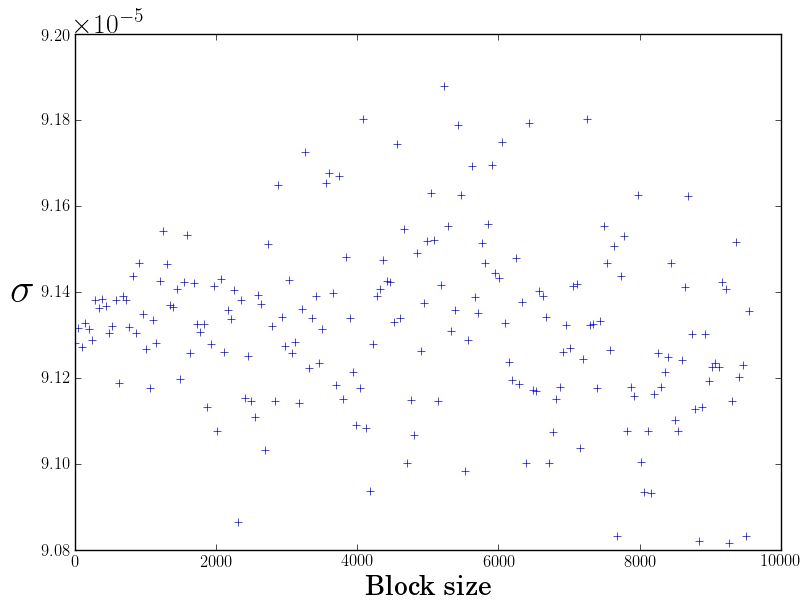
\includegraphics[scale=0.35]{../Graphics/BlockingExampleUncorr.png}}
  \subfigure{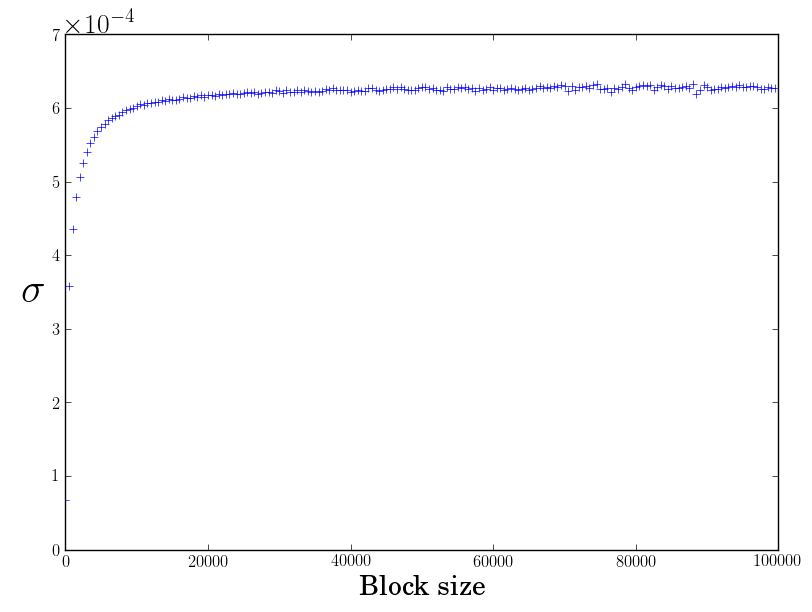
\includegraphics[scale=0.35]{../Graphics/BlockingExampleCorr.png}} 
  \caption{Left hand side: Blocking result of (approximately) uncorrelated data generated from a uniform Monte-Carlo integration of $\int _1^2 2x\mathrm{d}x$ resulting in $3.00003$ (exact is $3.0$). This is in excellent agreement with the magnitude of the error $\sim 9\cdot 10^{-5}$. There is no sign of a plateau, which implies fairly uncorrelated data (the span of the spread is small and apparently random). Right hand side: Blocking result of a DMC simulation of a 6-particle $\omega=0.1$ quantum dot. The plateau is strongly present, implying correlated data. The resulting total error is  $\sim 4.5\cdot 10^{-5}$.}
  \label{FIG:BlockingExamples}
 \end{center}
\end{figure}


\subsection{Variance Estimators}

The standard intuitive variance estimator

\begin{equation}
\label{eq:varBias}
 \sigma^2(x) \simeq \frac{1}{n}\sum_{i=1}^n (x_i - \overline{x})^2 = \left(\frac{1}{n}\sum_{i=1}^n x_i^2\right) - \overline{x}^2,
\end{equation}

is just an example of a variance estimator. A more precise estimator is 

\begin{equation}
\label{eq:varUnbias}
 \sigma^2(x) \simeq \frac{1}{n-1}\sum_{i=1}^n (x_i - \overline{x})^2 = \left(\frac{1}{n-1}\sum_{i=1}^n x_i^2\right) - \frac{n}{n-1}\overline{x}^2,
\end{equation}

which is only noticeably different from Eq.~(\ref{eq:varBias}) when the sample size gets small, as it does in blocking analysis. It is therefore standard to use Eq.~(\ref{eq:varUnbias}) for blocking errors.


